\documentclass[10pt, dvipdfmx]{beamer}
\AtBeginDvi{\special{pdf:tounicode 90ms-RKSJ-UCS2}}
\setbeamertemplate{navigation symbols}{}
\usetheme{default}
\setbeamertemplate{footline}[frame number]
\usefonttheme{professionalfonts}
\usepackage{helvet}
\usepackage{moreverb}
\renewcommand{\familydefault}{\sfdefault}
\renewcommand{\kanjifamilydefault}{\gtdefault}
\setbeamertemplate{caption}[numbered]

\title{tips (day5)}
\author{青木 聖也}
\institute[所属]{多摩美術大学情報デザイン研究室}
\date{August 8, 2017}

\uselanguage{japanese}
\languagepath{japanese}

\begin{document}
    \begin{frame}[plain]
        \frametitle{}
	    \titlepage
    \end{frame}

    \begin{frame}
        \frametitle{Contents}
        \tableofcontents
    \end{frame}

%-----------------------------------------------------------
% 1日目1限:アプリ間通信紹介
    \section{まずはじめに}
        \begin{frame}
            \frametitle{資料について}
            \begin{columns}[c]
                \begin{column}{0.80\textwidth}
                    \begin{block}{今回の資料を以下に公開しています}
                        \begin{itemize}
                            \scriptsize
                            \item 全体説明: http://scottallen.ws/tamabi/summerworkshop2017
                            \item スライド: https://github.com/5c0tt411en/iddsummerworkshop2017/blob/master/Slide/
                        \end{itemize}
                    \end{block}
                \end{column}
            \end{columns}
        \end{frame}

    \section{展示の自動化について}
    \subsection{macOS自動起動・シャットダウン}
        \begin{frame}
            \frametitle{macOS自動起動・シャットダウン}
            \begin{block}{自動起動の利点}
                \begin{itemize}
                    \item 仕様書にて学芸員やスタッフの方に起動してもらう必要がない
                    \item 立ち上げ・立ち下げ忘れなどのミスがない
                \end{itemize}
            \end{block}
        \end{frame}

        \begin{frame}
            \frametitle{macOS自動起動・シャットダウン}
                \begin{figure}[htb]
                    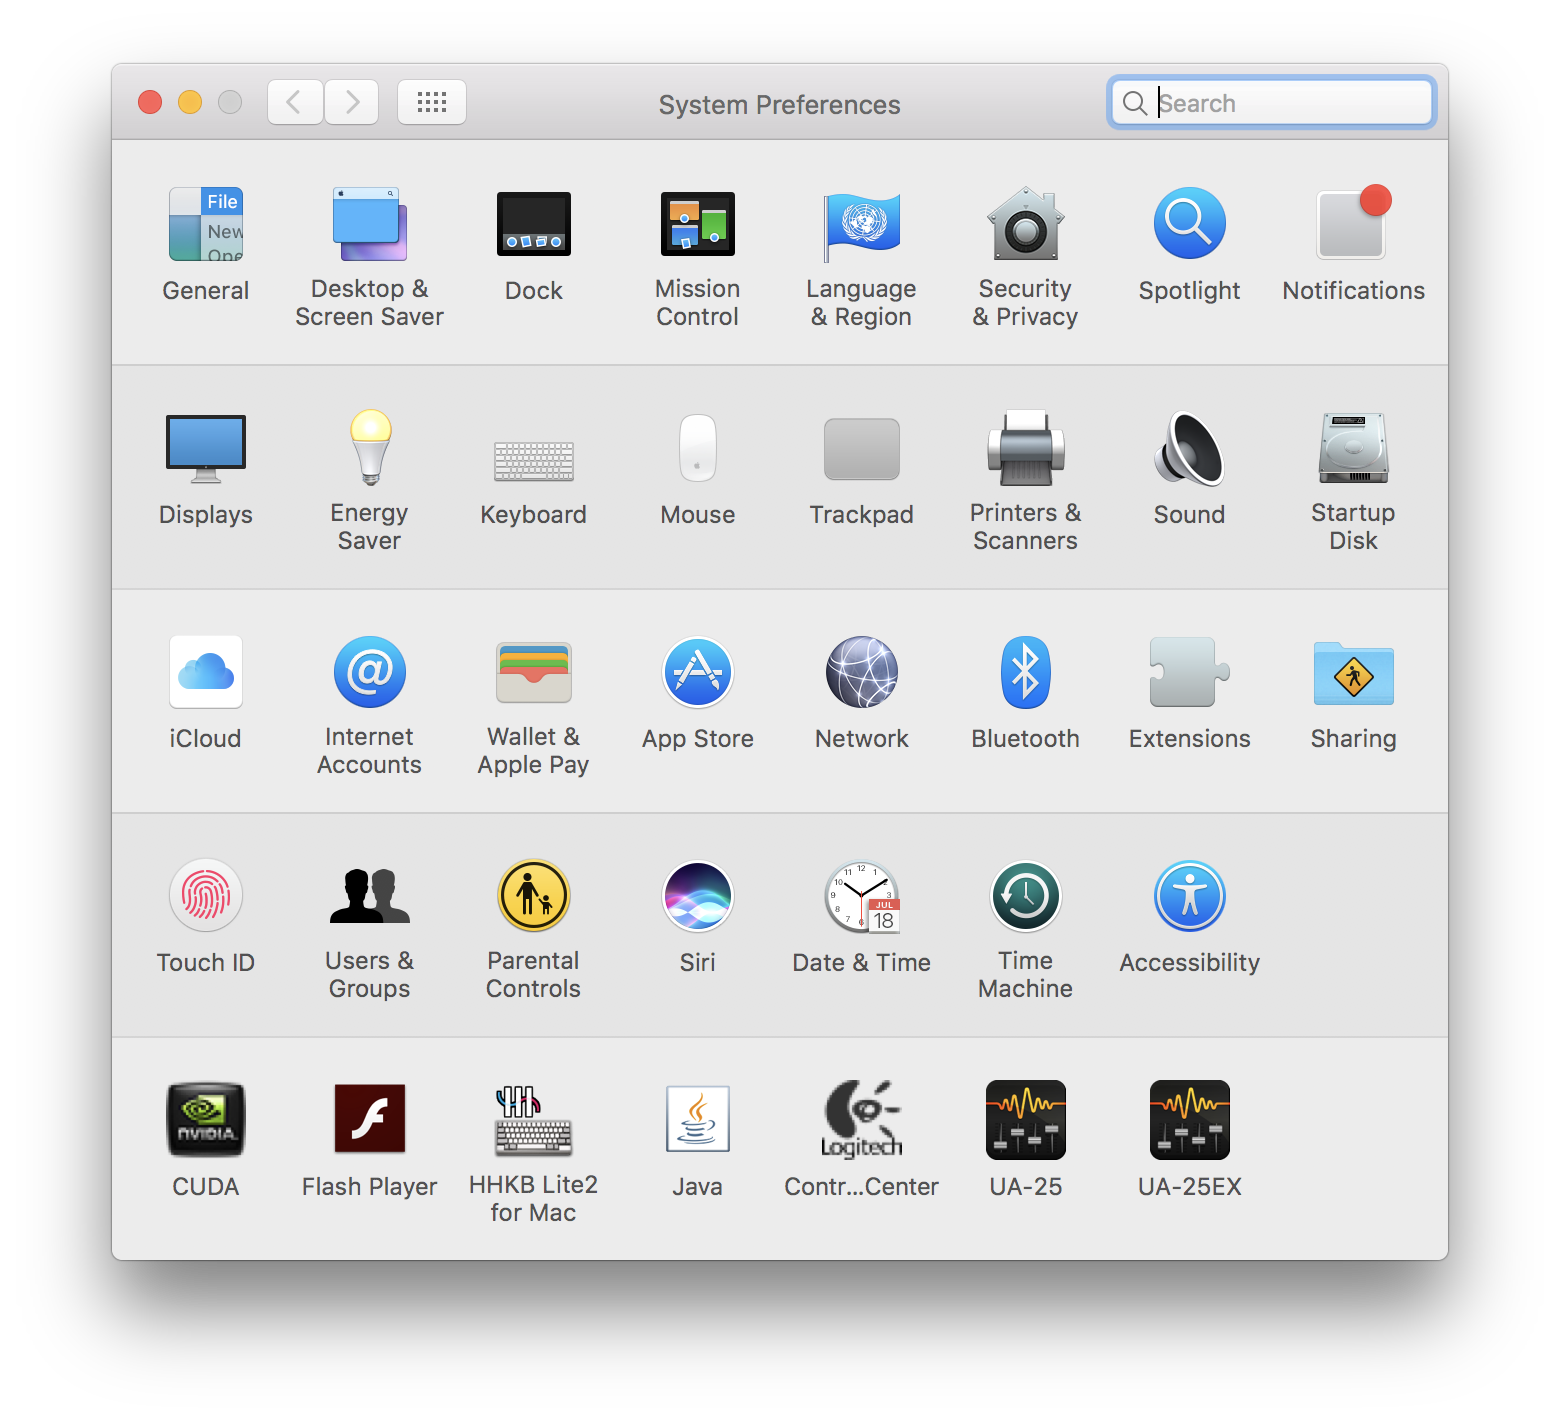
\includegraphics[width=70mm]{images/auto-1.png}
                    \caption{システム環境設定}
                    \label{fig:01}
                \end{figure}
        \end{frame}

        \begin{frame}
            \frametitle{macOS自動起動・シャットダウン}
                \begin{figure}[htb]
                    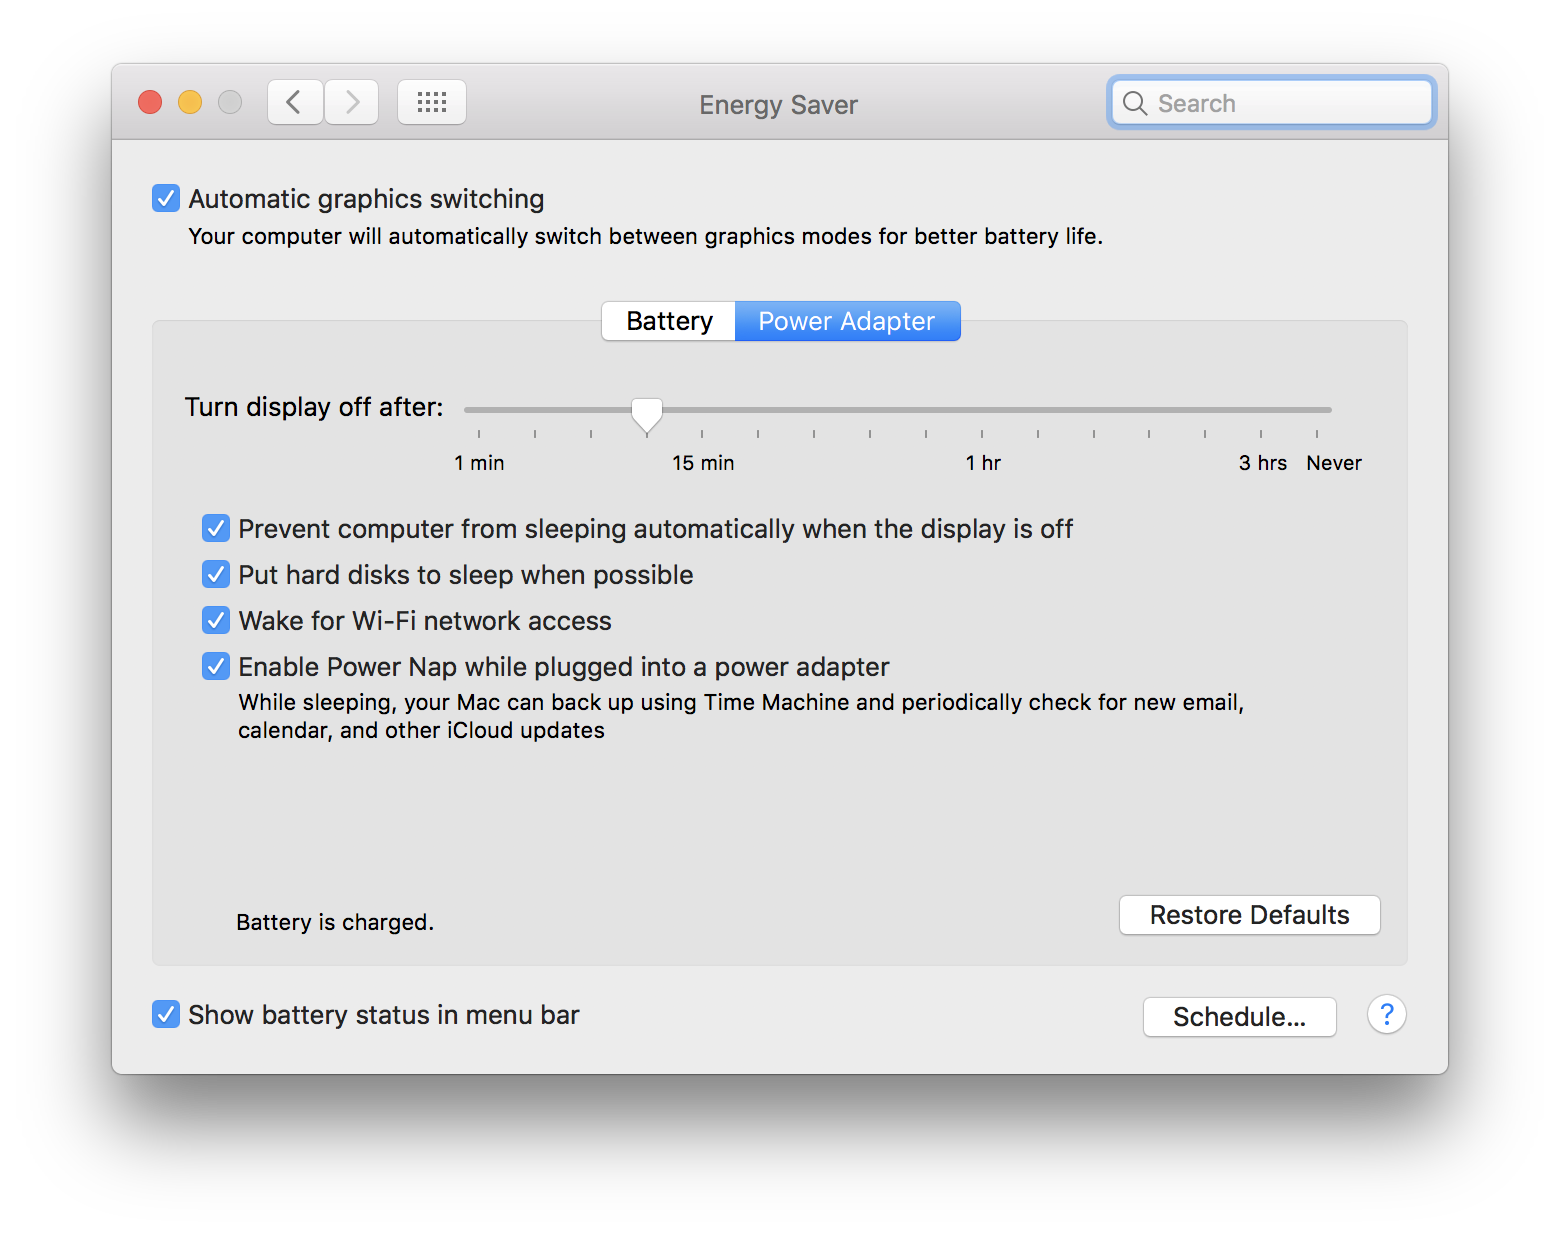
\includegraphics[width=70mm]{images/auto-2.png}
                    \caption{省エネルギー}
                    \label{fig:02}
                \end{figure}
        \end{frame}

        \begin{frame}
            \frametitle{macOS自動起動・シャットダウン}
                \begin{figure}[htb]
                    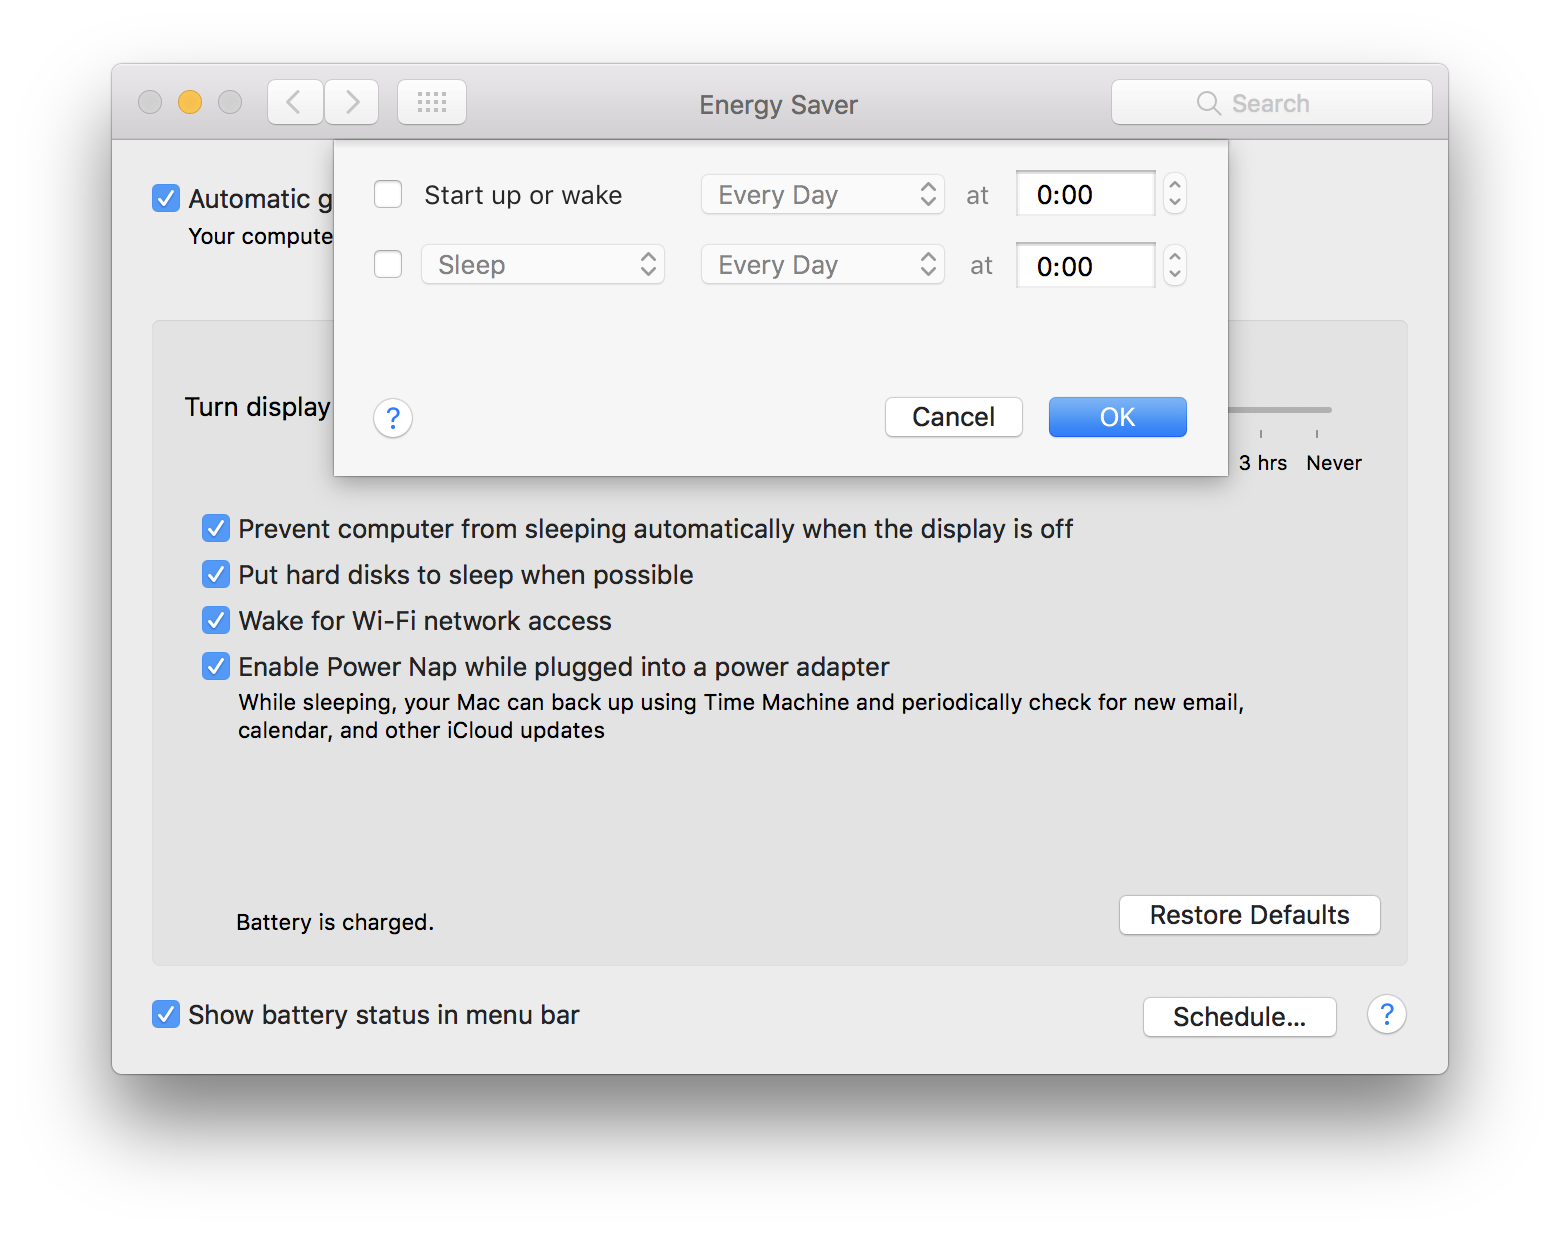
\includegraphics[width=70mm]{images/auto-3.png}
                    \caption{スケジュール}
                    \label{fig:03}
                \end{figure}
        \end{frame}

        \begin{frame}
            \frametitle{macOS自動起動・シャットダウン}
                \begin{figure}[htb]
                    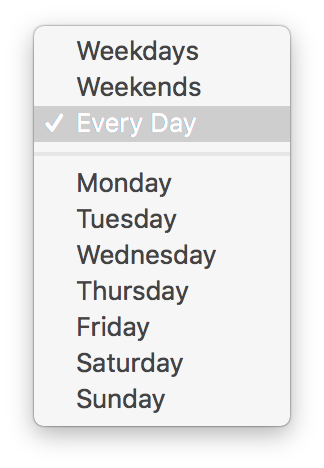
\includegraphics[width=20mm]{images/auto-4.png}
                    \caption{頻度設定}
                    \label{fig:04}
                \end{figure}
        \end{frame}

        \begin{frame}
            \frametitle{macOS自動起動・シャットダウン}
                \begin{figure}[htb]
                    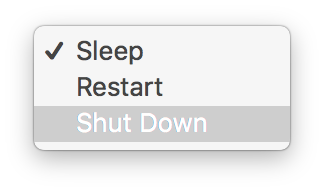
\includegraphics[width=20mm]{images/auto-5.png}
                    \caption{シャットダウン設定}
                    \label{fig:05}
                \end{figure}
        \end{frame}

        \begin{frame}
            \frametitle{macOS自動起動・シャットダウン}
                \begin{figure}[htb]
                    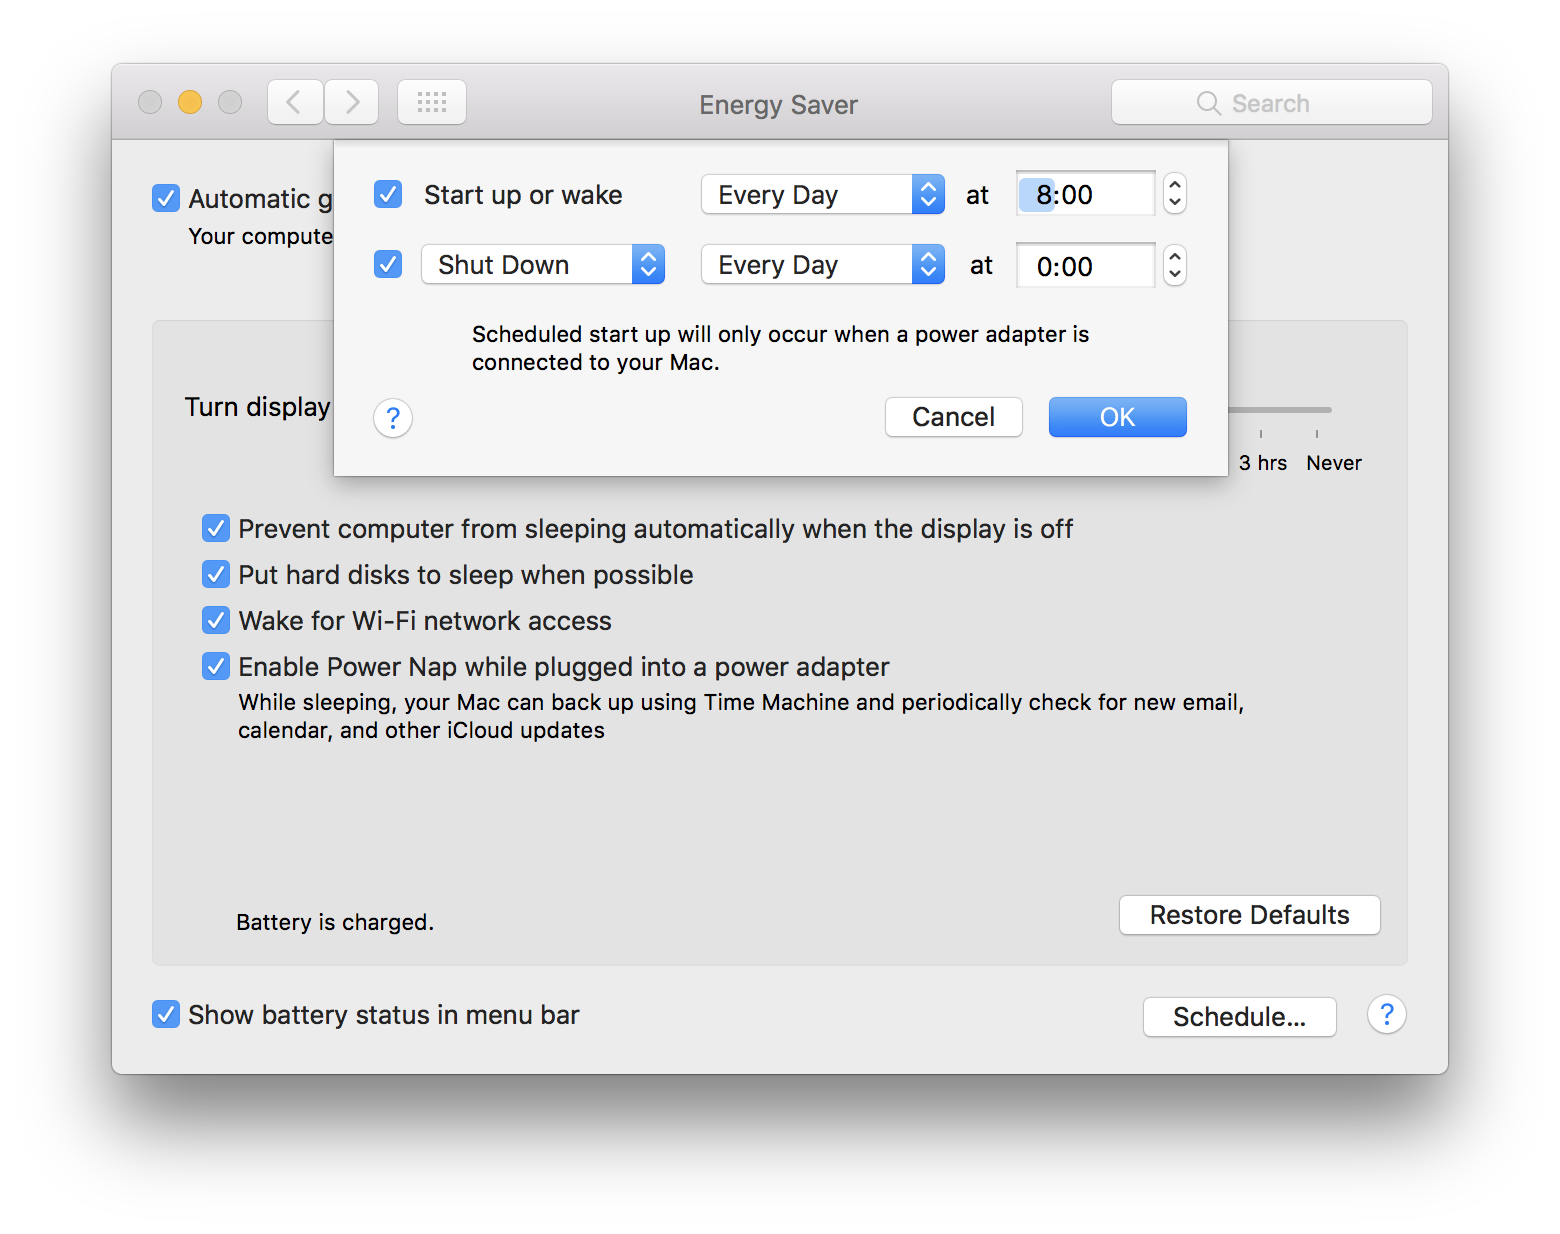
\includegraphics[width=70mm]{images/auto-6.png}
                    \caption{最終画面}
                    \label{fig:06}
                \end{figure}
        \end{frame}

    \subsection{アプリの自動起動・終了}
        \begin{frame}
            \frametitle{アプリの自動起動・終了}
            \begin{block}{アプリ自動起動・終了の意義}
                \begin{itemize}
                    \item 決まった時間に決まったアプリによって処理を実行できる
                    \item アプリ起動の順番を指定してうまく連携できる
                \end{itemize}
            \end{block}
        \end{frame}

        \begin{frame}
            \frametitle{アプリの自動起動・終了}
                \begin{figure}[htb]
                    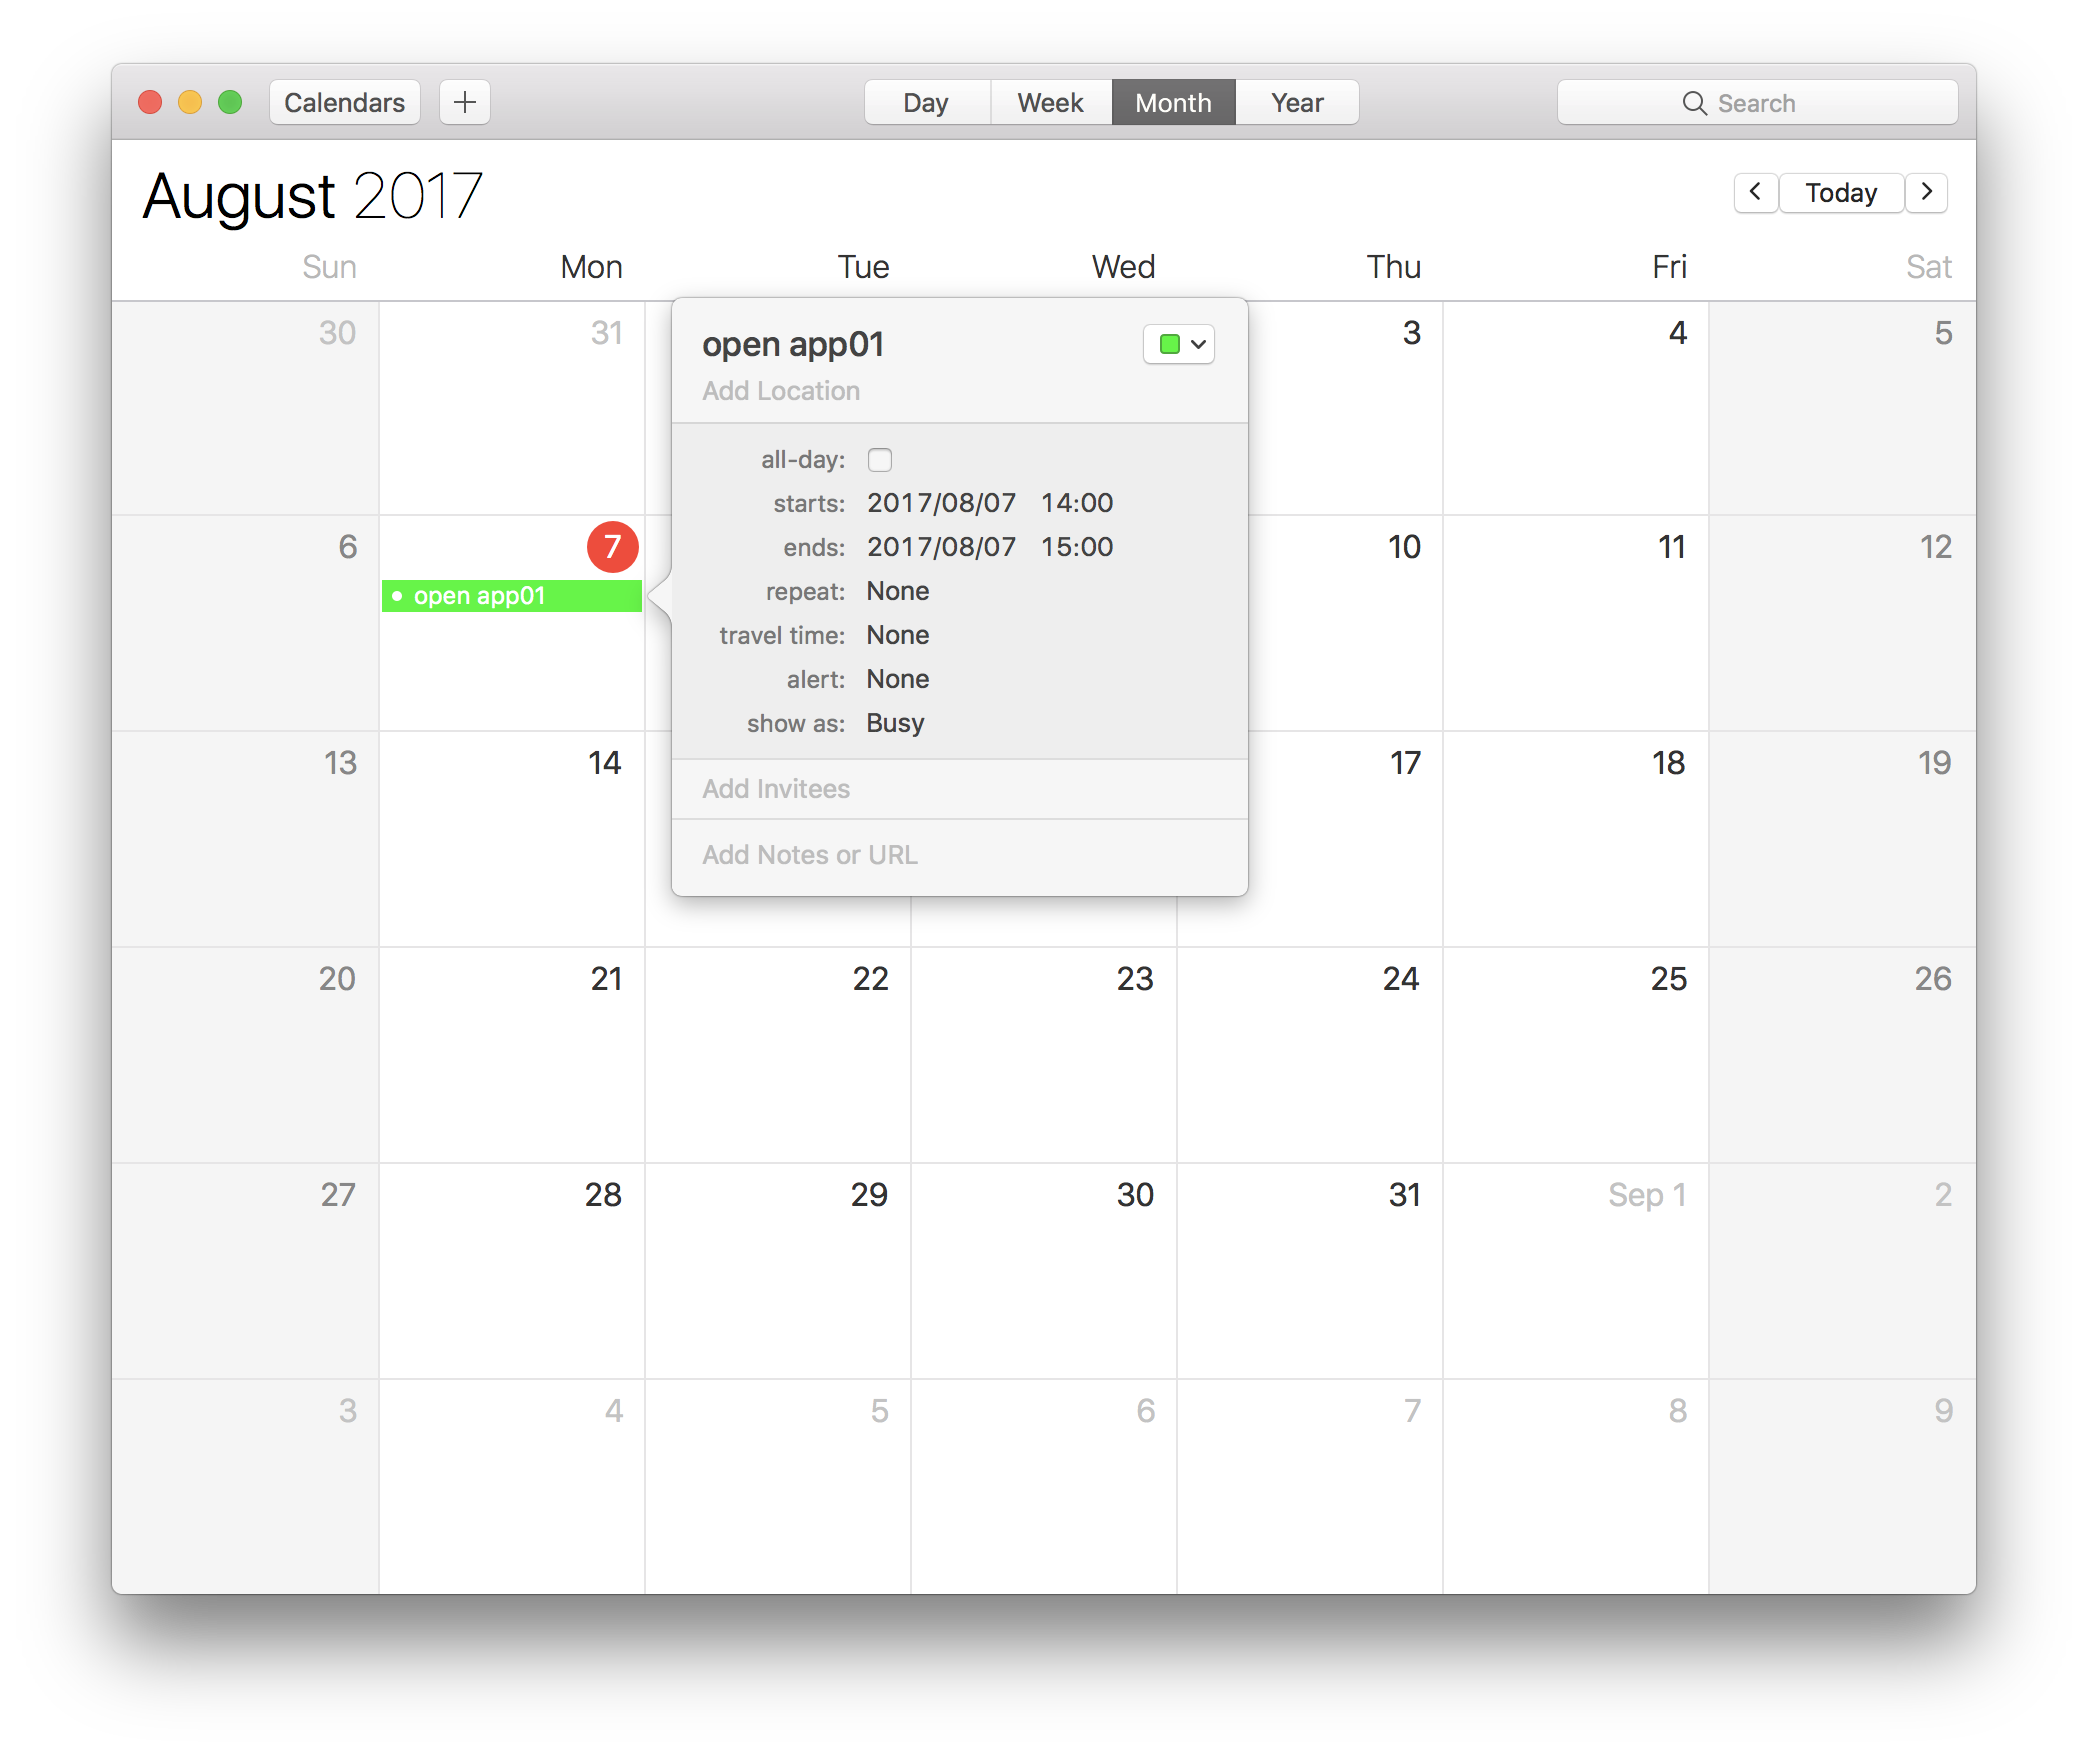
\includegraphics[width=70mm]{images/app-1.png}
                    \caption{新規予定作成}
                    \label{fig:08}
                \end{figure}
        \end{frame}

        \begin{frame}
            \frametitle{アプリの自動起動・終了}
                \begin{figure}[htb]
                    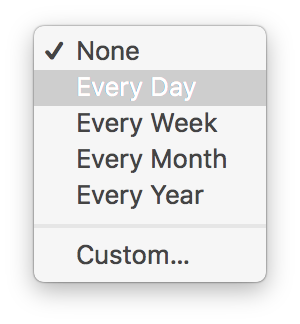
\includegraphics[width=20mm]{images/app-2.png}
                    \caption{繰り返しを設定}
                    \label{fig:09}
                \end{figure}
        \end{frame}

        \begin{frame}
            \frametitle{アプリの自動起動・終了}
                \begin{figure}[htb]
                    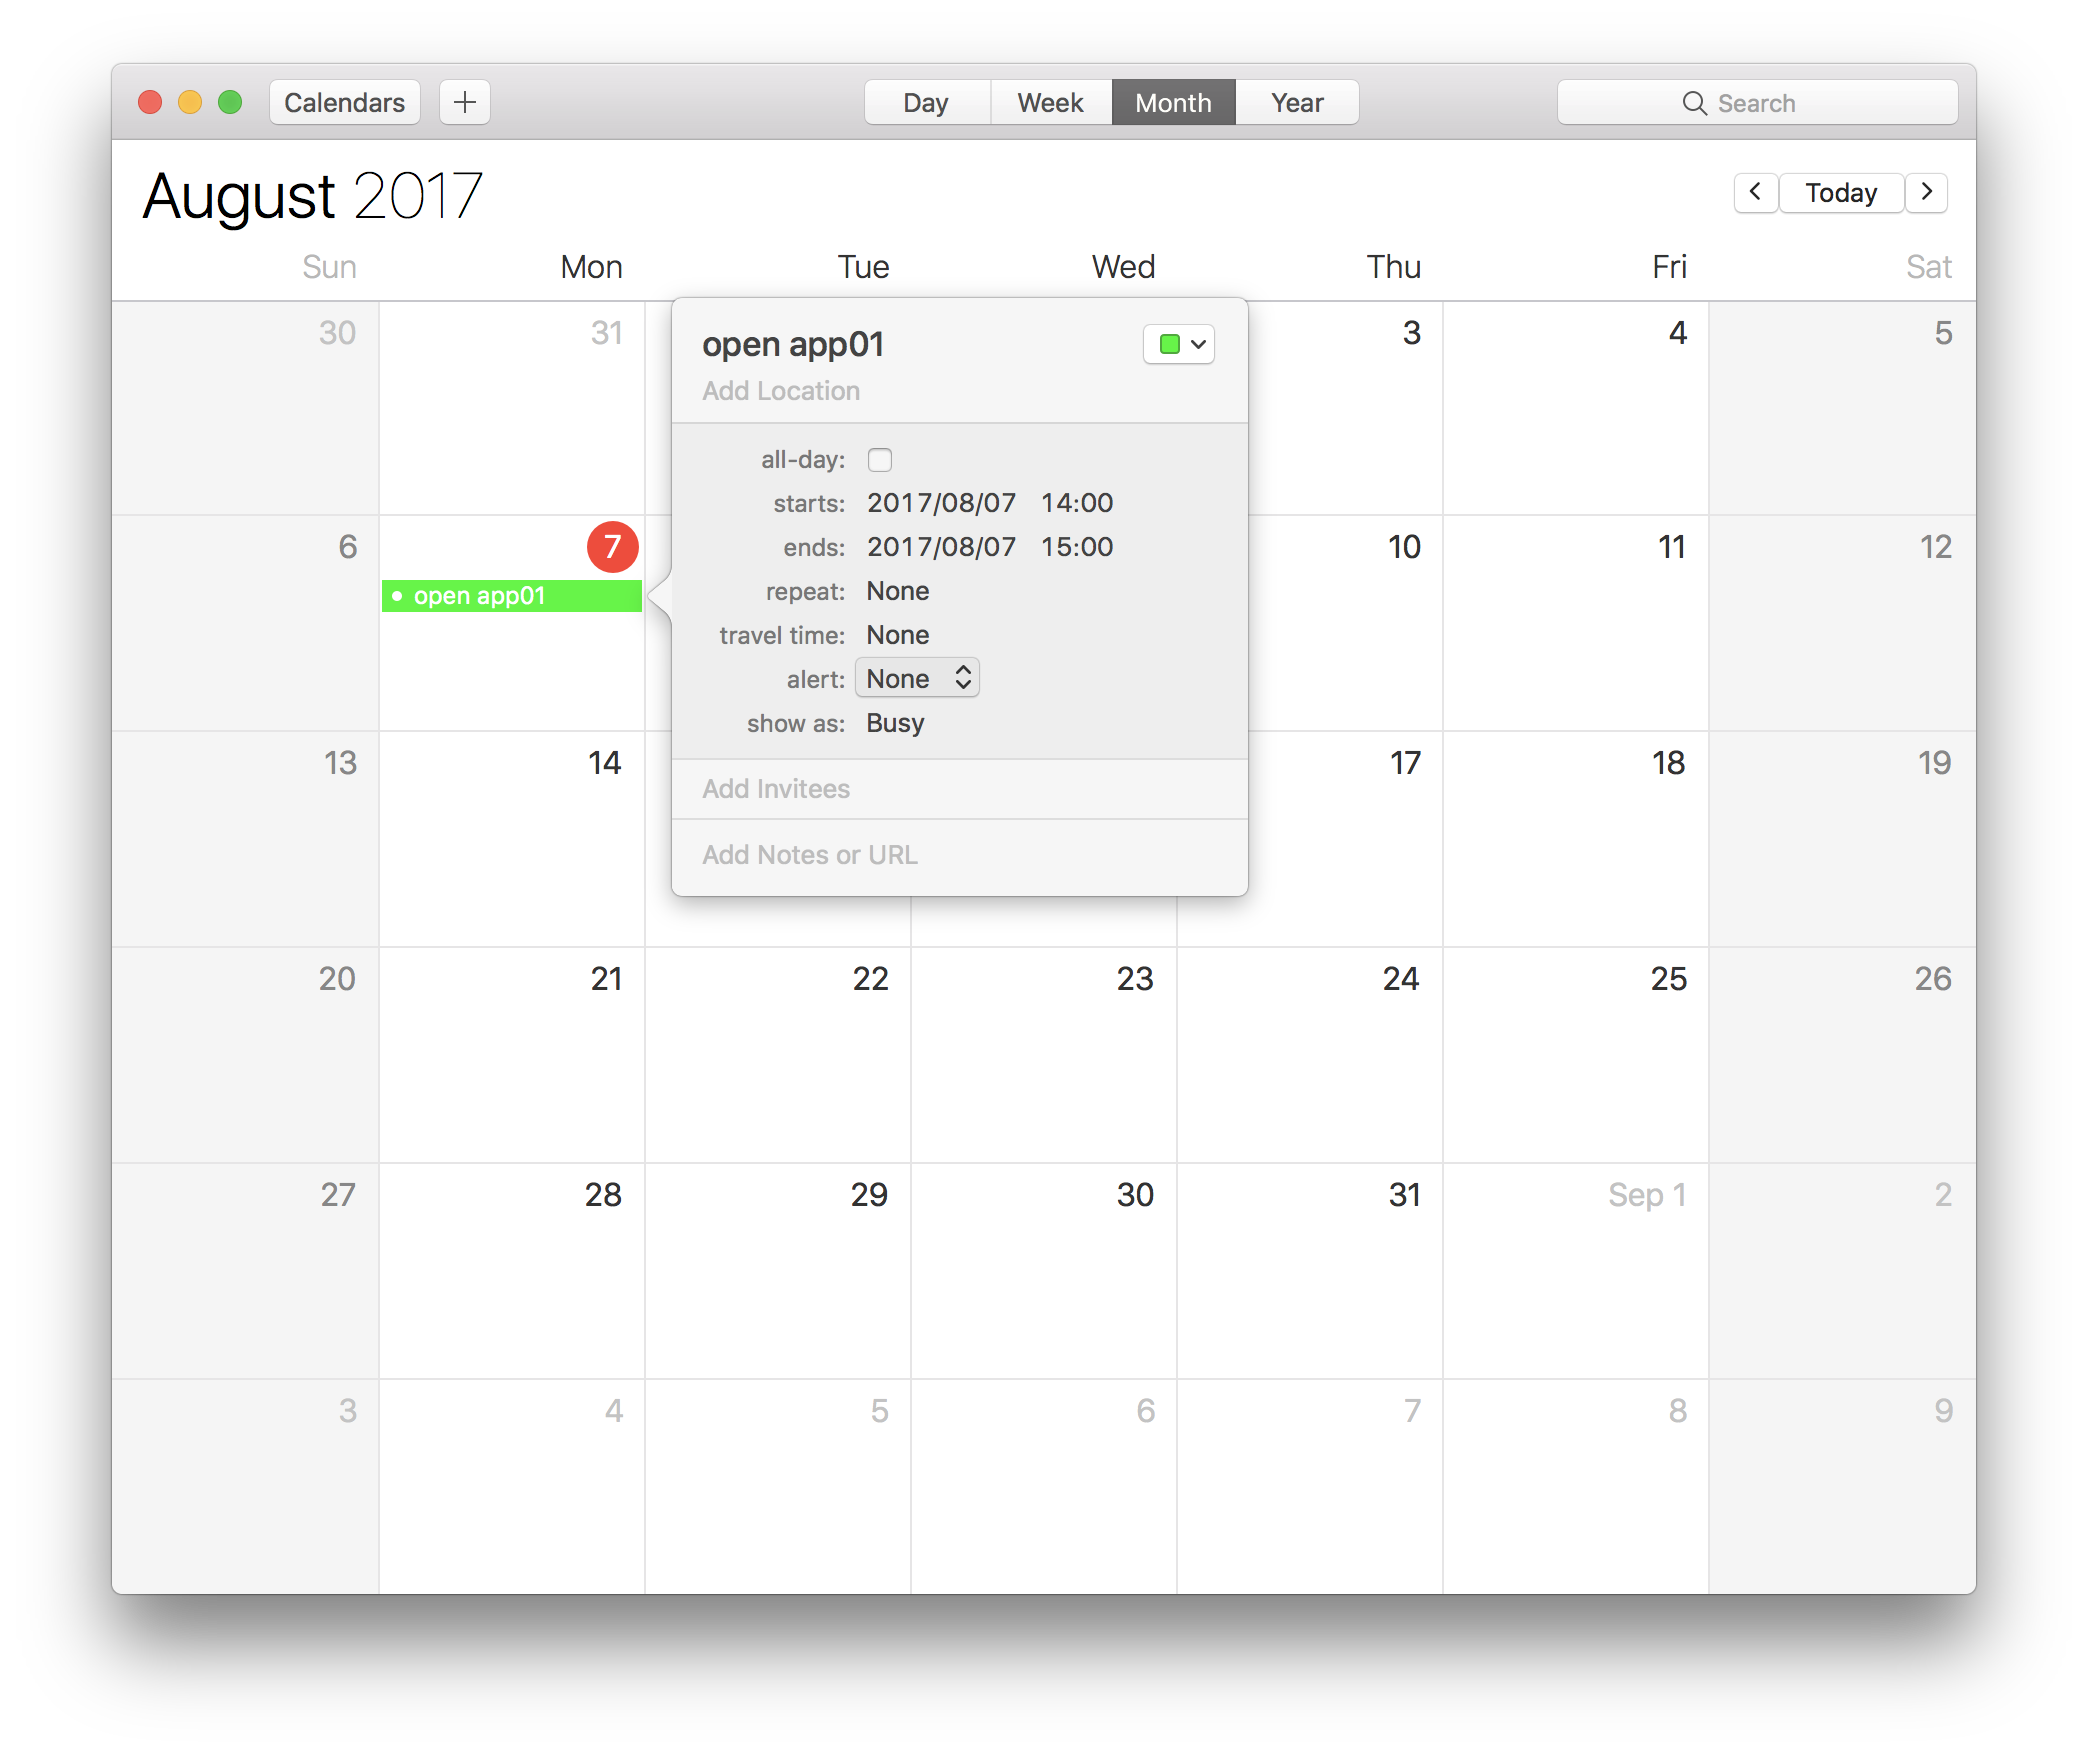
\includegraphics[width=70mm]{images/app-3.png}
                    \caption{通知を選択}
                    \label{fig:10}
                \end{figure}
        \end{frame}

        \begin{frame}
            \frametitle{アプリの自動起動・終了}
                \begin{figure}[htb]
                    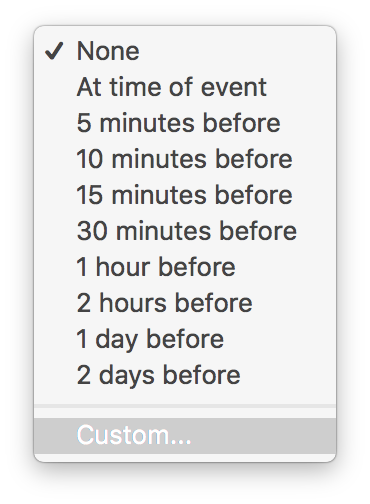
\includegraphics[width=20mm]{images/app-4.png}
                    \caption{カスタムを選択}
                    \label{fig:11}
                \end{figure}
        \end{frame}

        \begin{frame}
            \frametitle{アプリの自動起動・終了}
                \begin{figure}[htb]
                    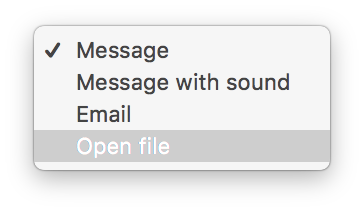
\includegraphics[width=20mm]{images/app-5.png}
                    \caption{ファイルを開くを選択}
                    \label{fig:12}
                \end{figure}
        \end{frame}

        \begin{frame}
            \frametitle{アプリの自動起動・終了}
                \begin{figure}[htb]
                    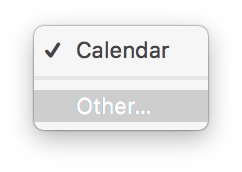
\includegraphics[width=20mm]{images/app-6.png}
                    \caption{その他}
                    \label{fig:13}
                \end{figure}
        \end{frame}

        \begin{frame}
            \frametitle{アプリの自動起動・終了}
                \begin{figure}[htb]
                    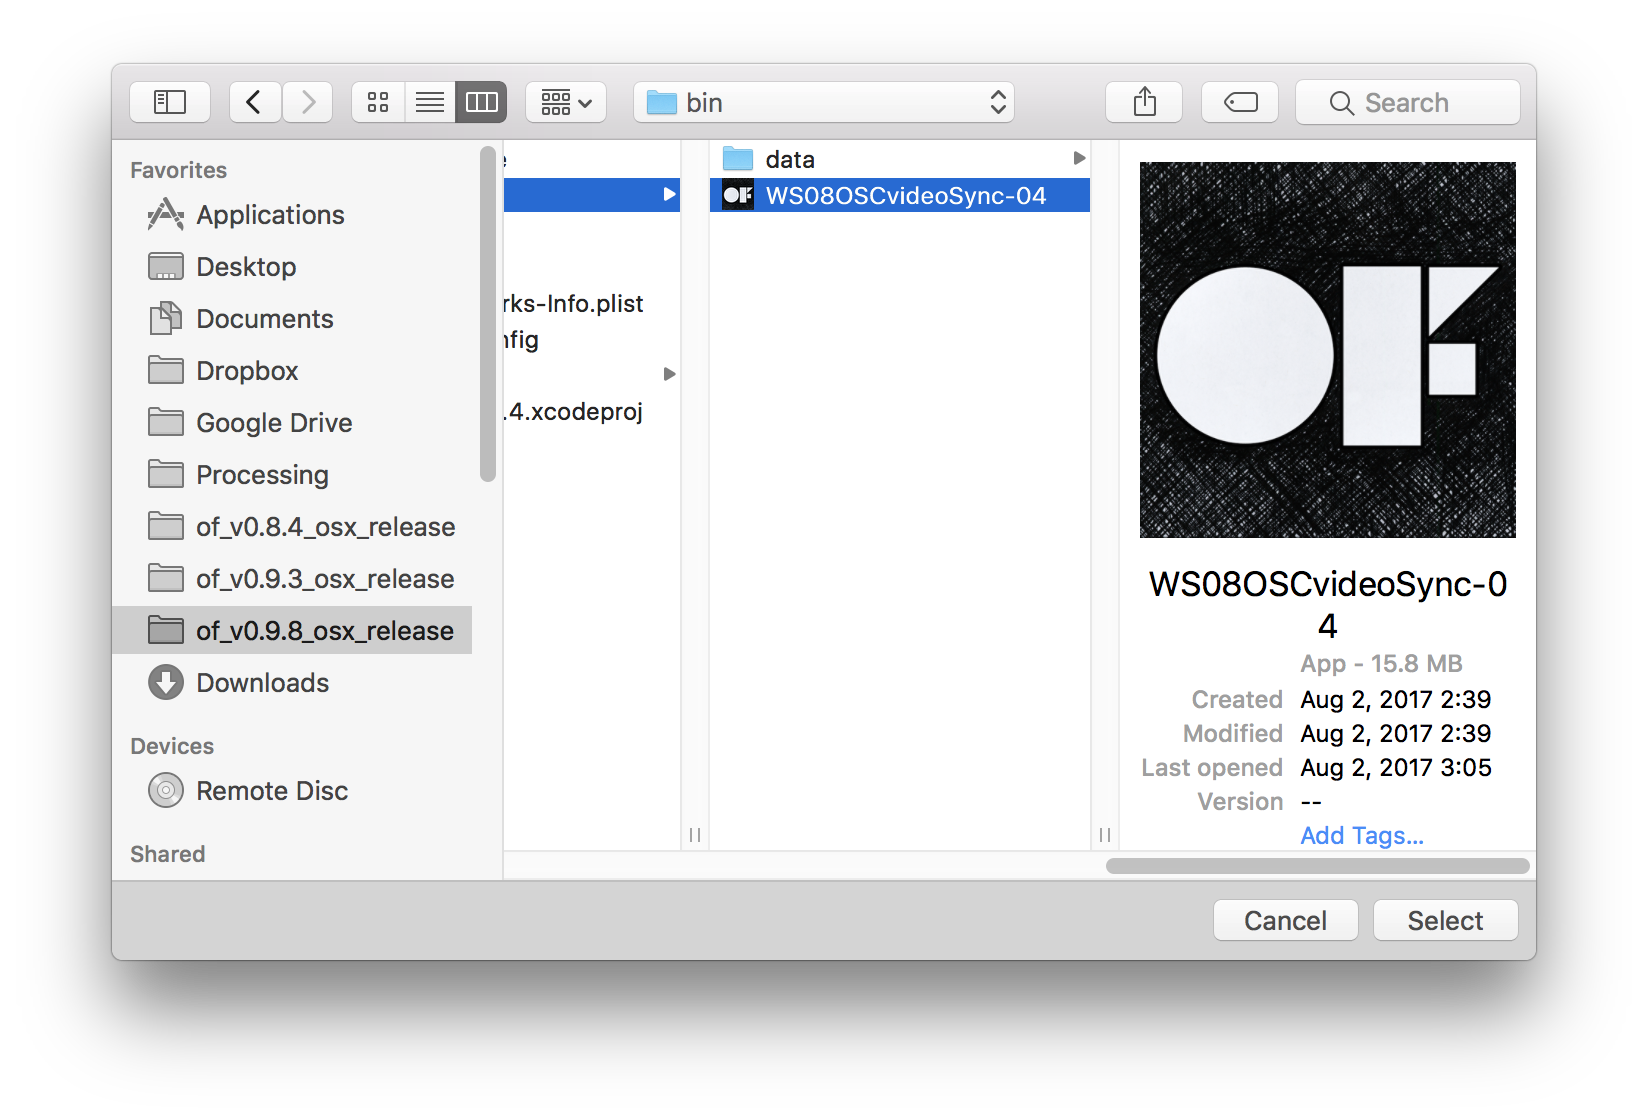
\includegraphics[width=70mm]{images/app-7.png}
                    \caption{立ち上げたい制作したアプリを選択}
                    \label{fig:14}
                \end{figure}
        \end{frame}

        \begin{frame}
            \frametitle{アプリの自動起動・終了}
                \begin{figure}[htb]
                    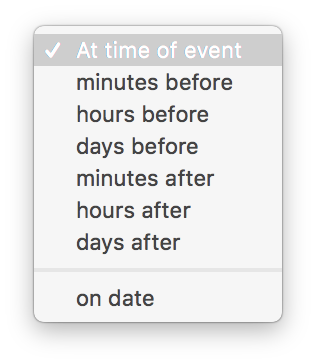
\includegraphics[width=20mm]{images/app-8.png}
                    \caption{イベントの時間に設定}
                    \label{fig:15}
                \end{figure}
        \end{frame}

        \begin{frame}
            \frametitle{アプリの自動起動・終了}
                \begin{figure}[htb]
                    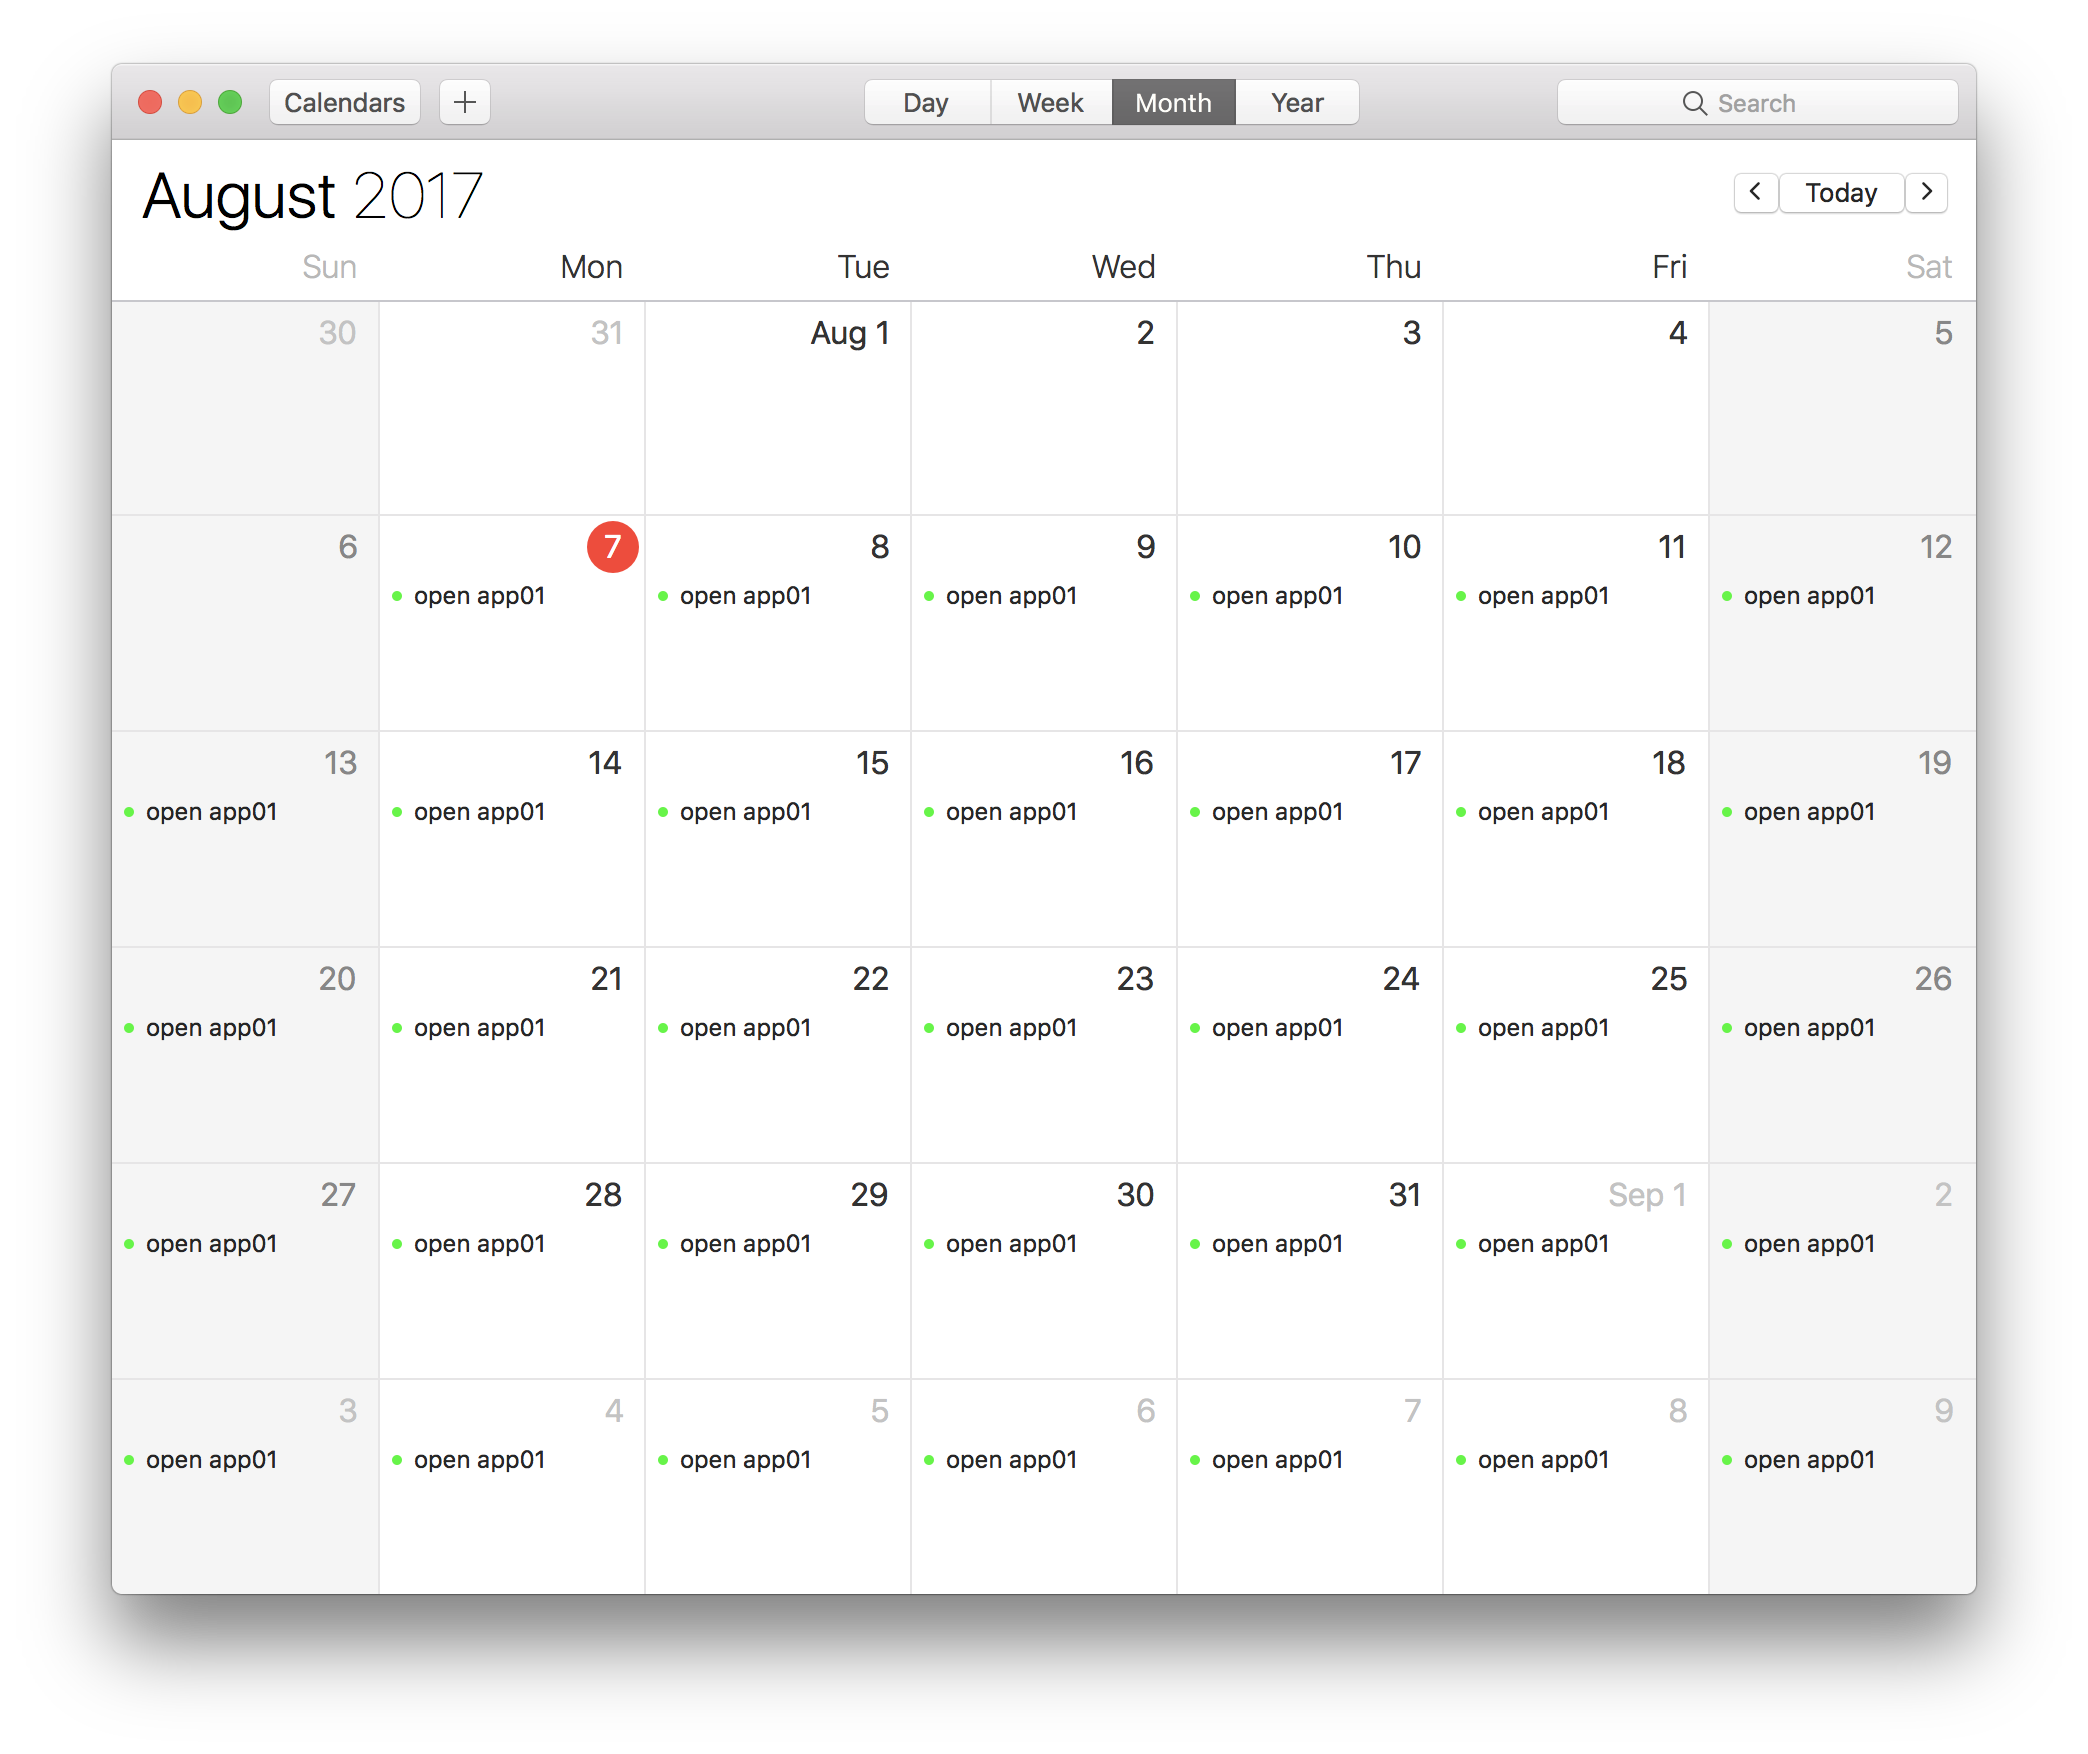
\includegraphics[width=70mm]{images/app-9.png}
                    \caption{結果}
                    \label{fig:16}
                \end{figure}
        \end{frame}

        \begin{frame}
            \frametitle{アプリの自動起動・終了}
                \begin{figure}[htb]
                    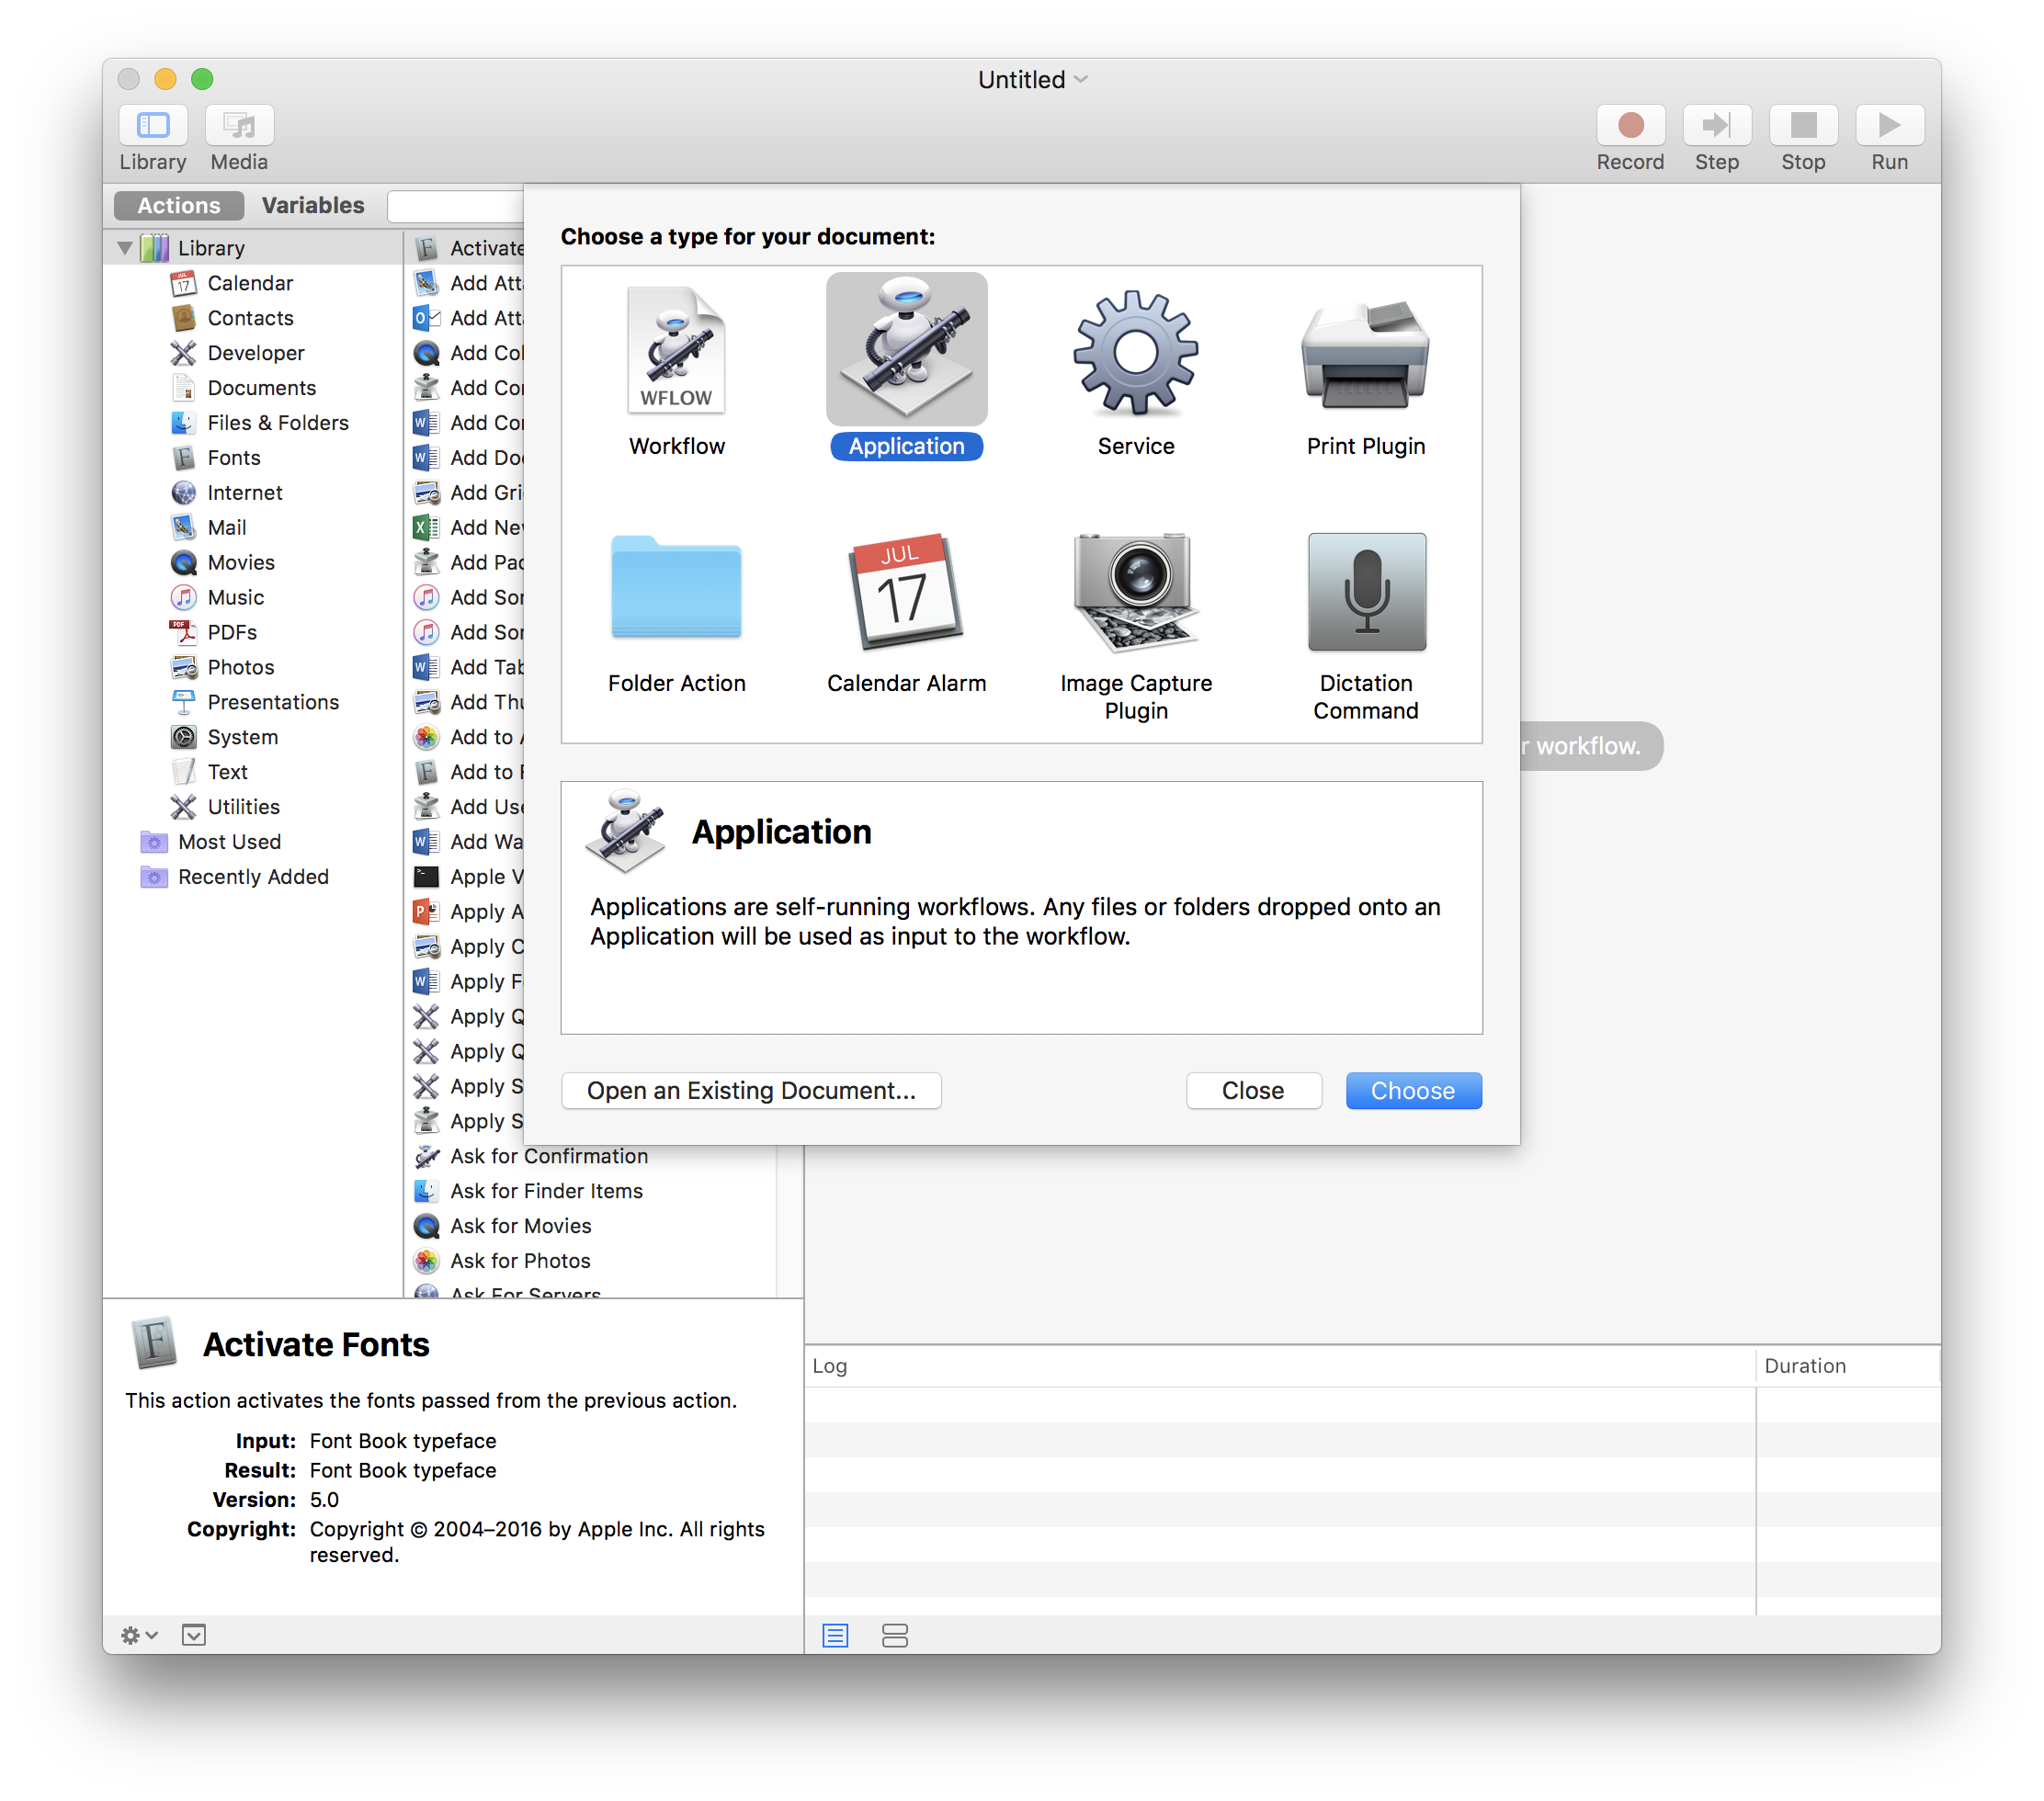
\includegraphics[width=70mm]{images/app-10.png}
                    \caption{automatorを開く}
                    \label{fig:17}
                \end{figure}
        \end{frame}

        \begin{frame}
            \frametitle{アプリの自動起動・終了}
                \begin{figure}[htb]
                    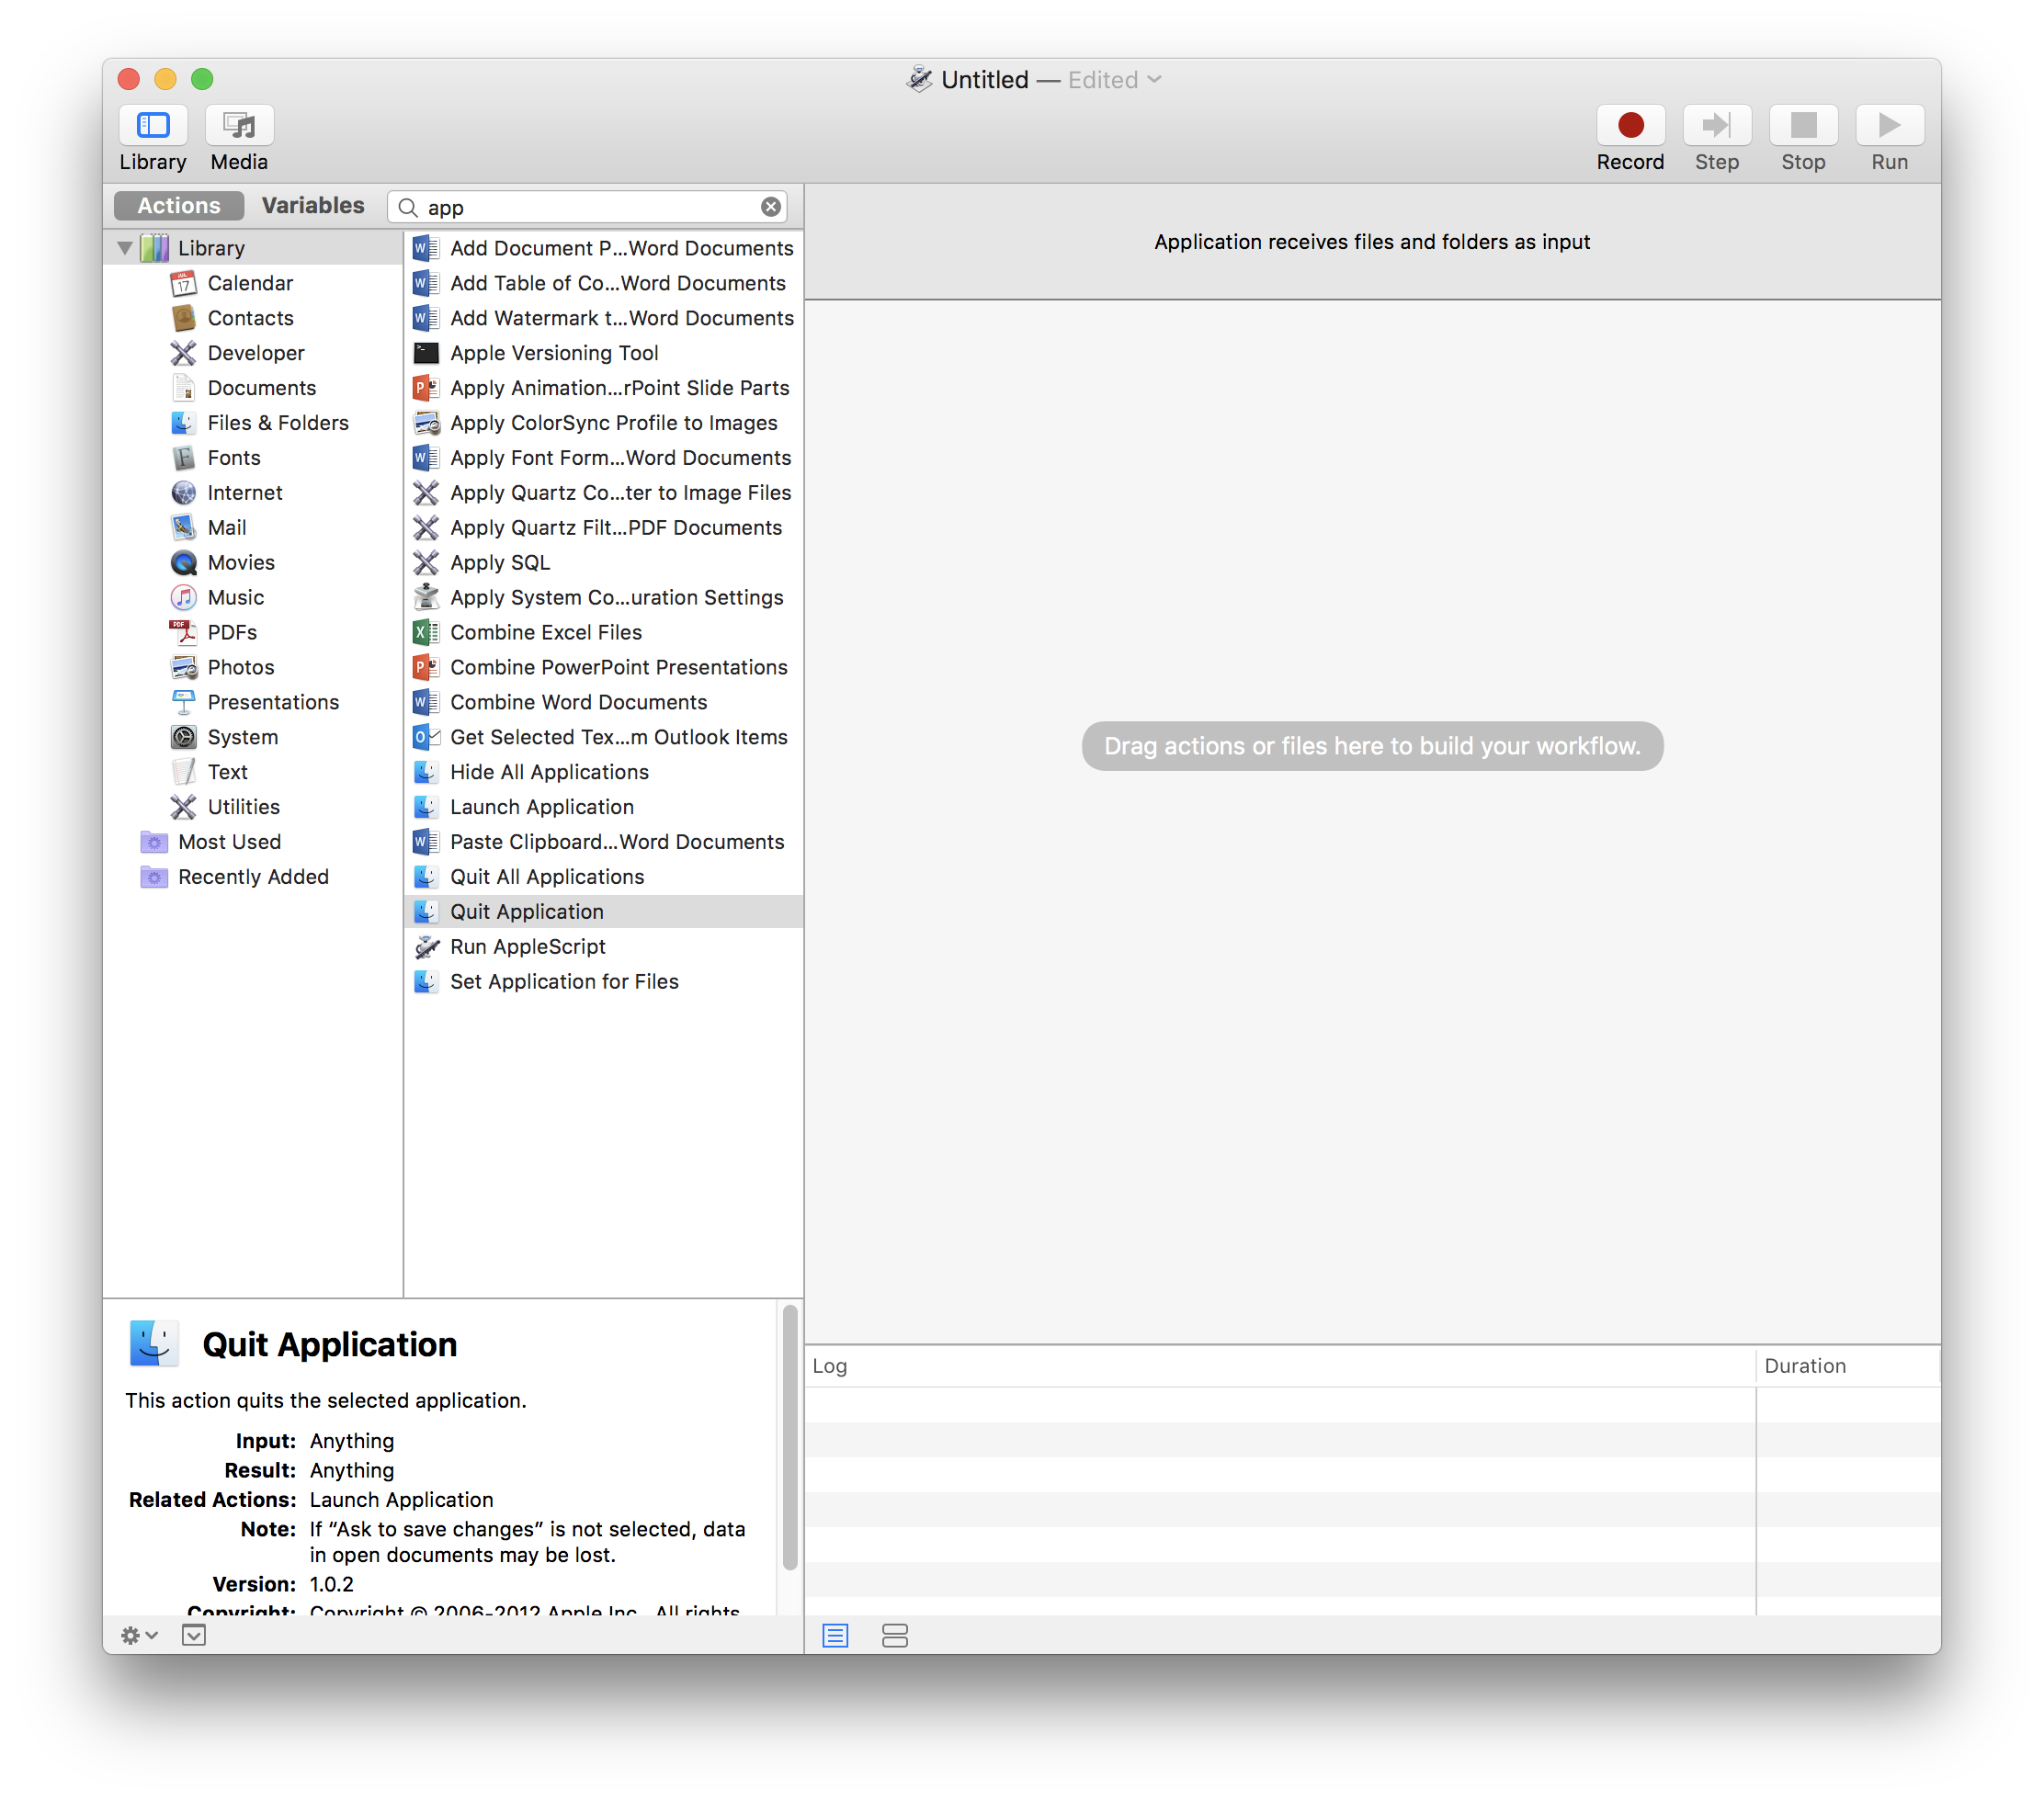
\includegraphics[width=70mm]{images/app-11.png}
                    \caption{アプリの終了を選択}
                    \label{fig:18}
                \end{figure}
        \end{frame}

        \begin{frame}
            \frametitle{アプリの自動起動・終了}
                \begin{figure}[htb]
                    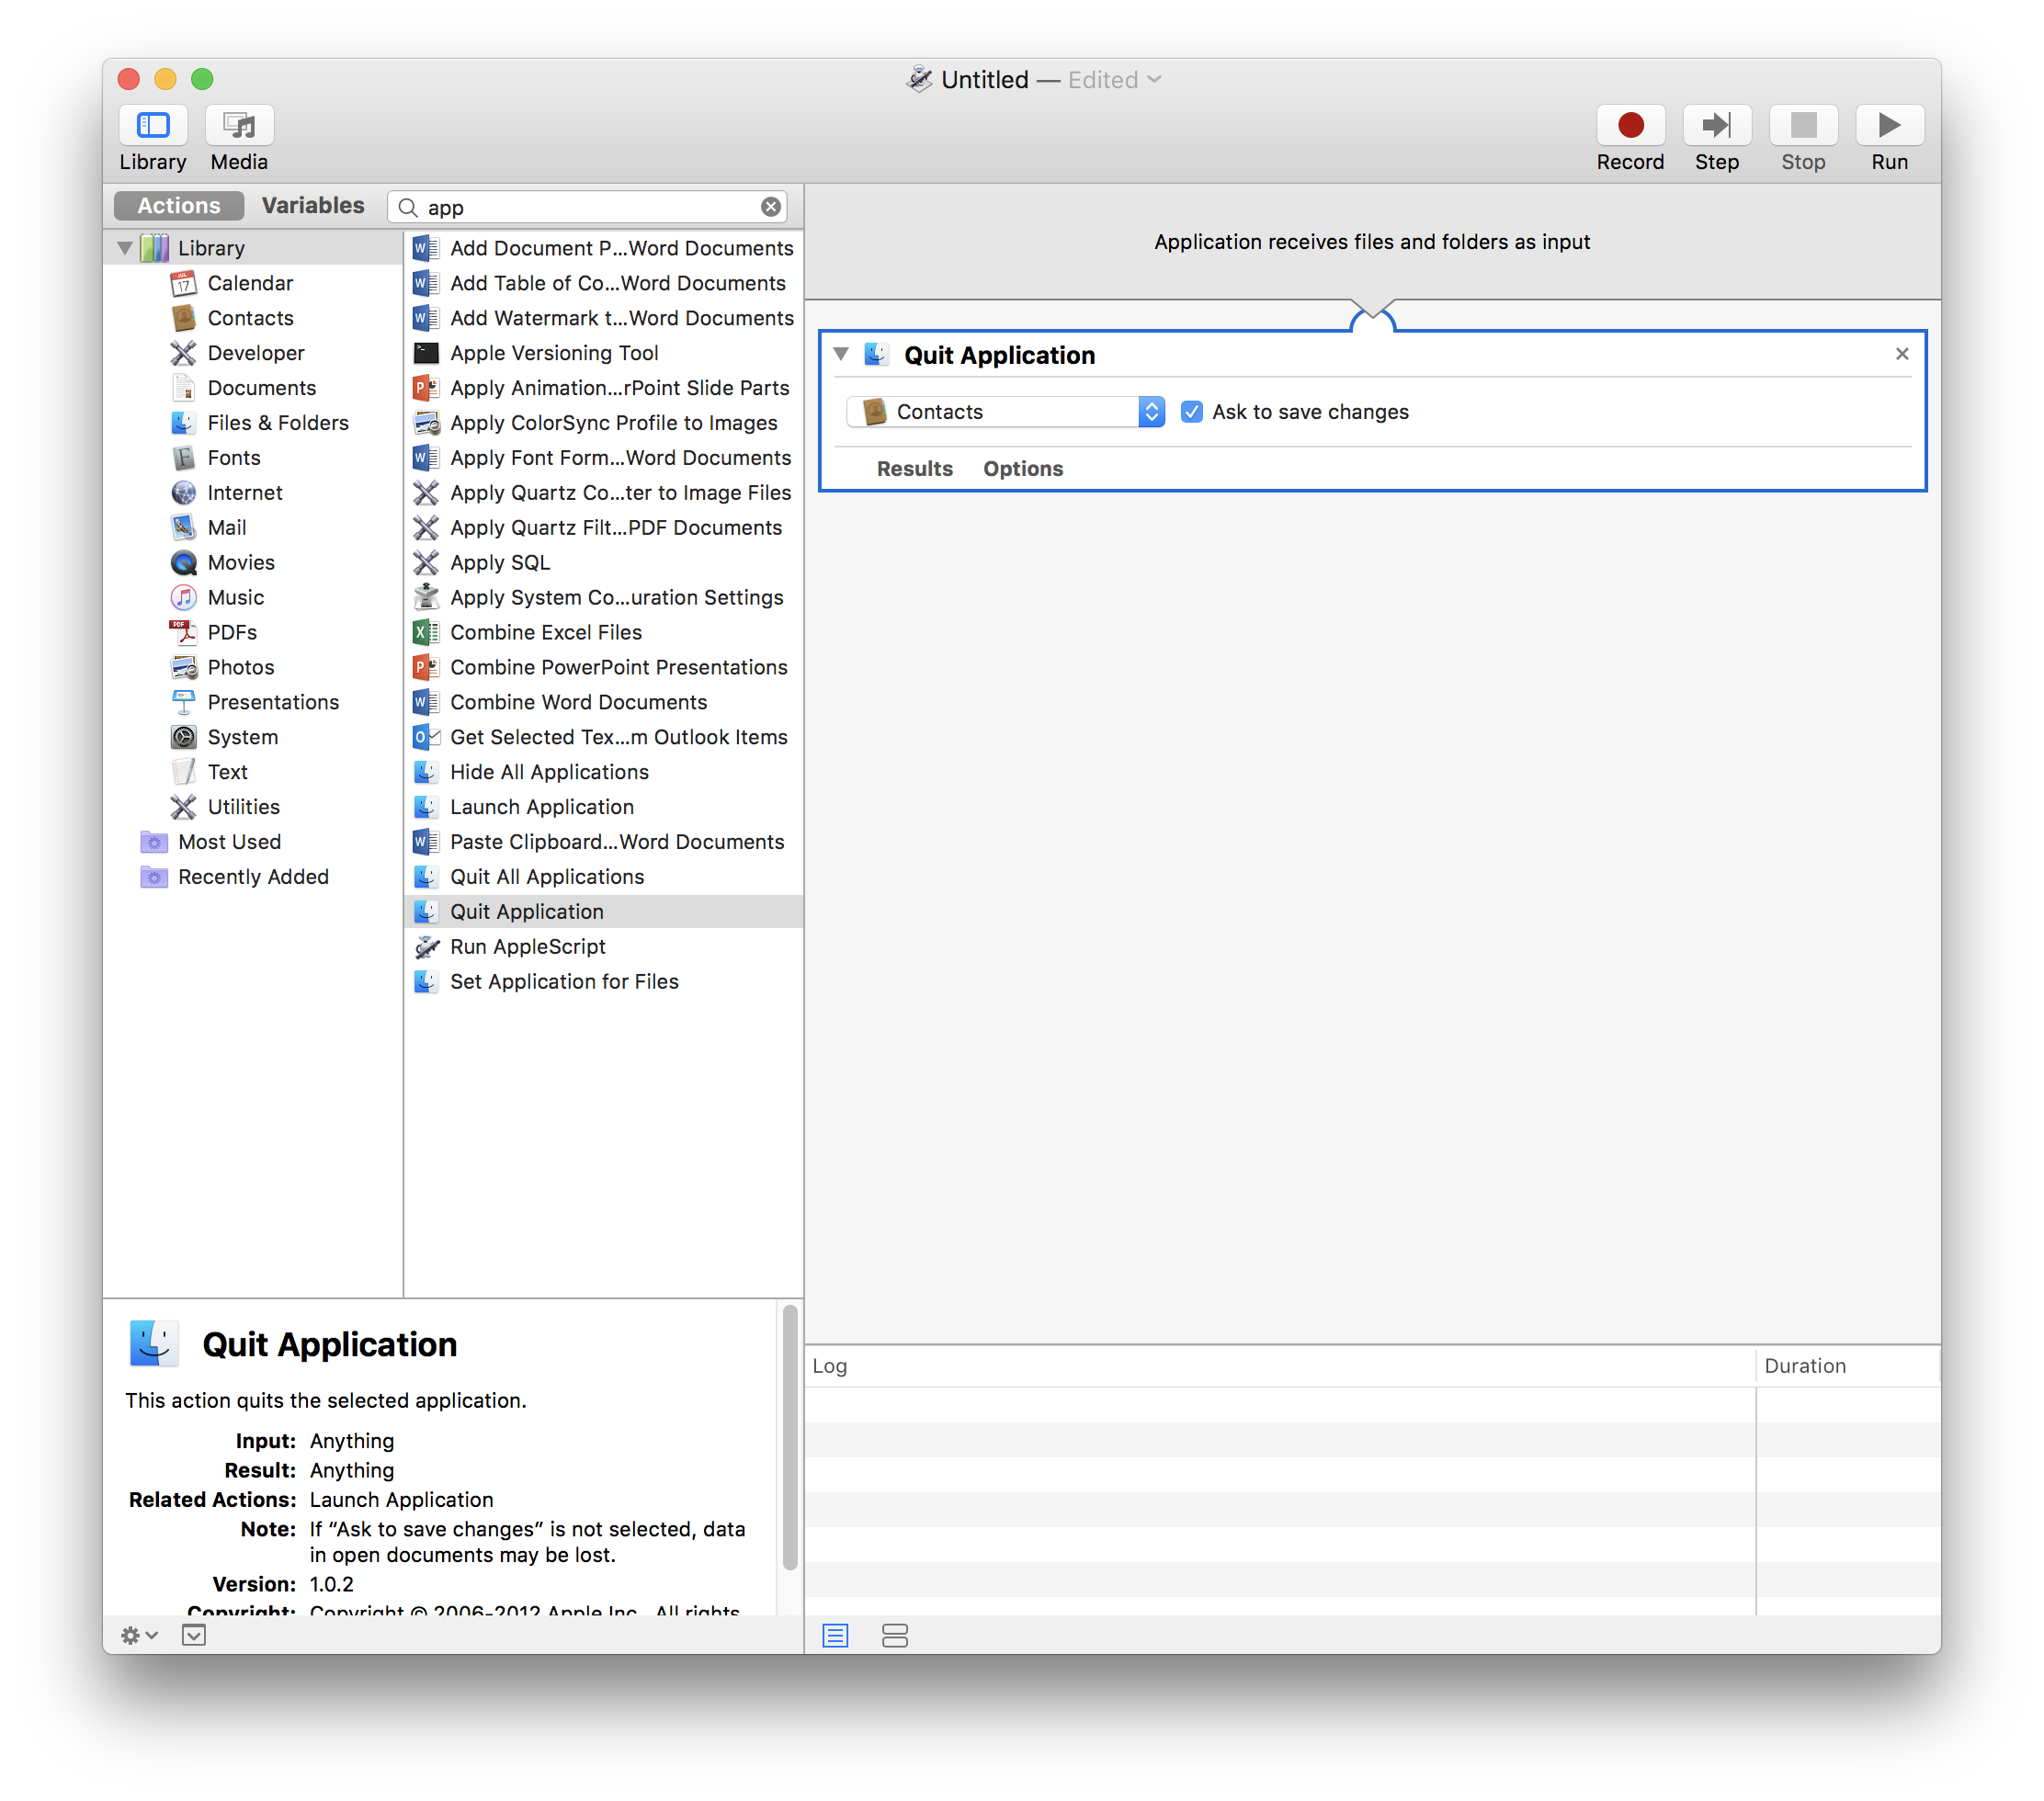
\includegraphics[width=70mm]{images/app-12.png}
                    \caption{結果}
                    \label{fig:19}
                \end{figure}
        \end{frame}

        \begin{frame}
            \frametitle{アプリの自動起動・終了}
                \begin{figure}[htb]
                    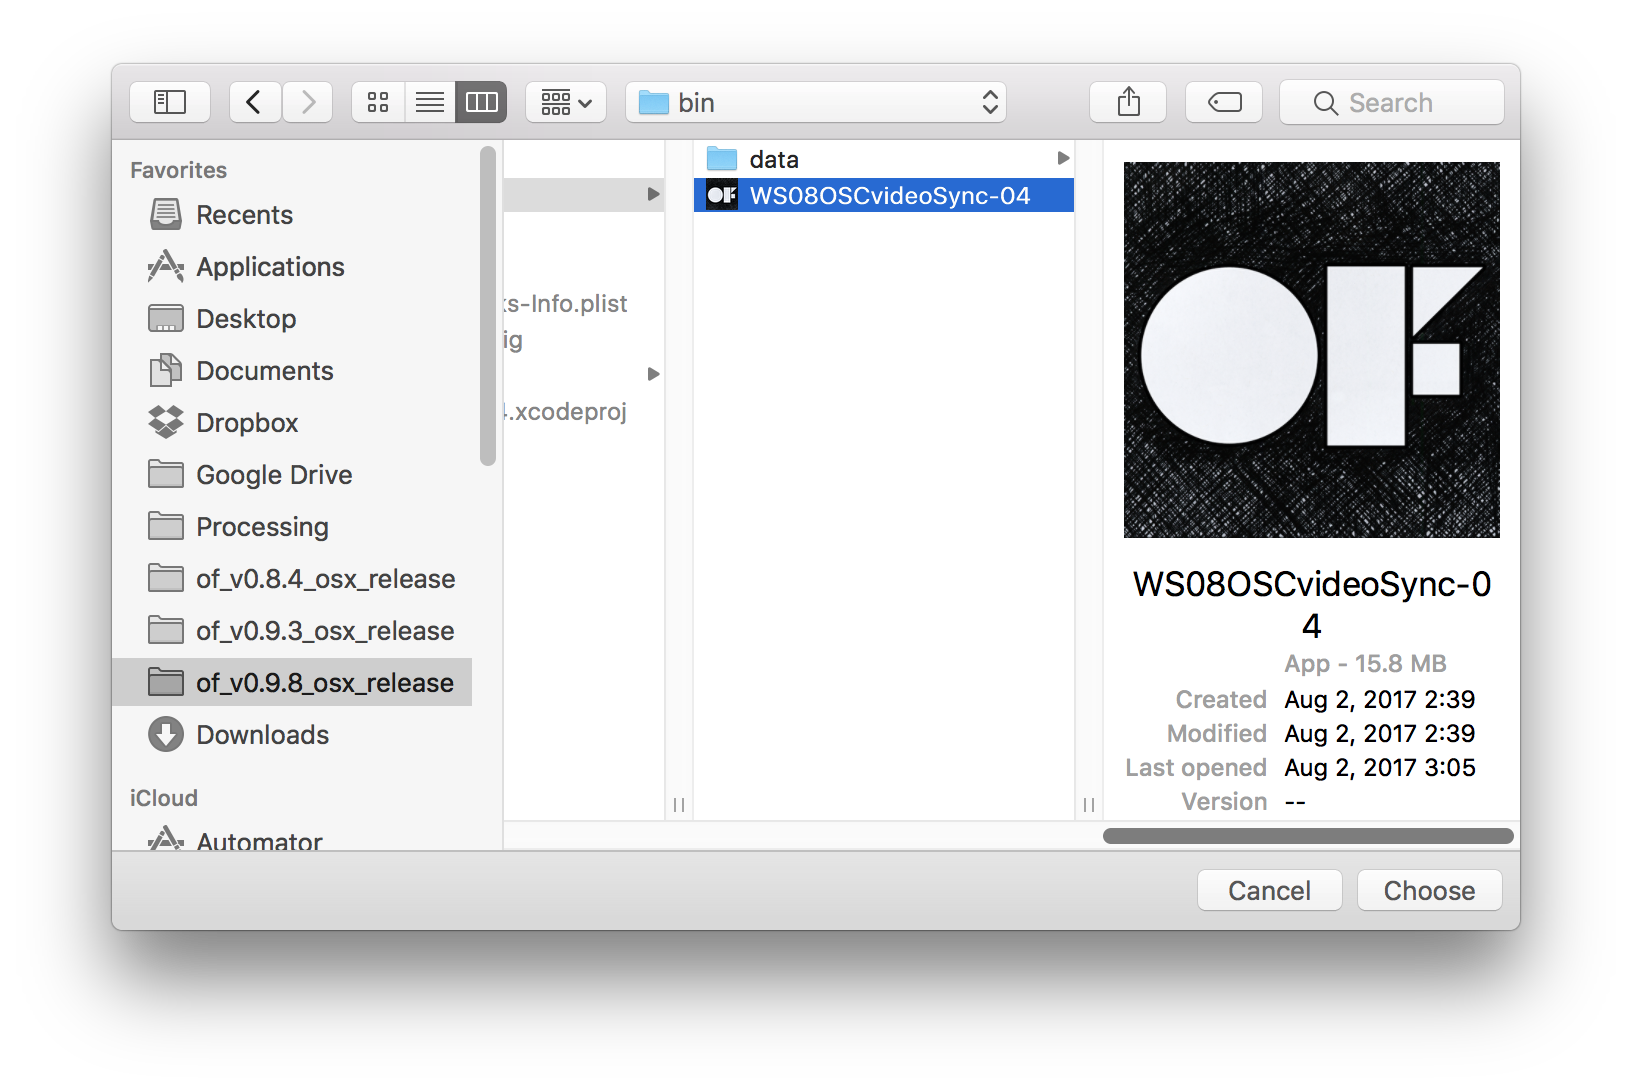
\includegraphics[width=70mm]{images/app-13.png}
                    \caption{終了するアプリを選択}
                    \label{fig:20}
                \end{figure}
        \end{frame}

        \begin{frame}
            \frametitle{アプリの自動起動・終了}
                \begin{figure}[htb]
                    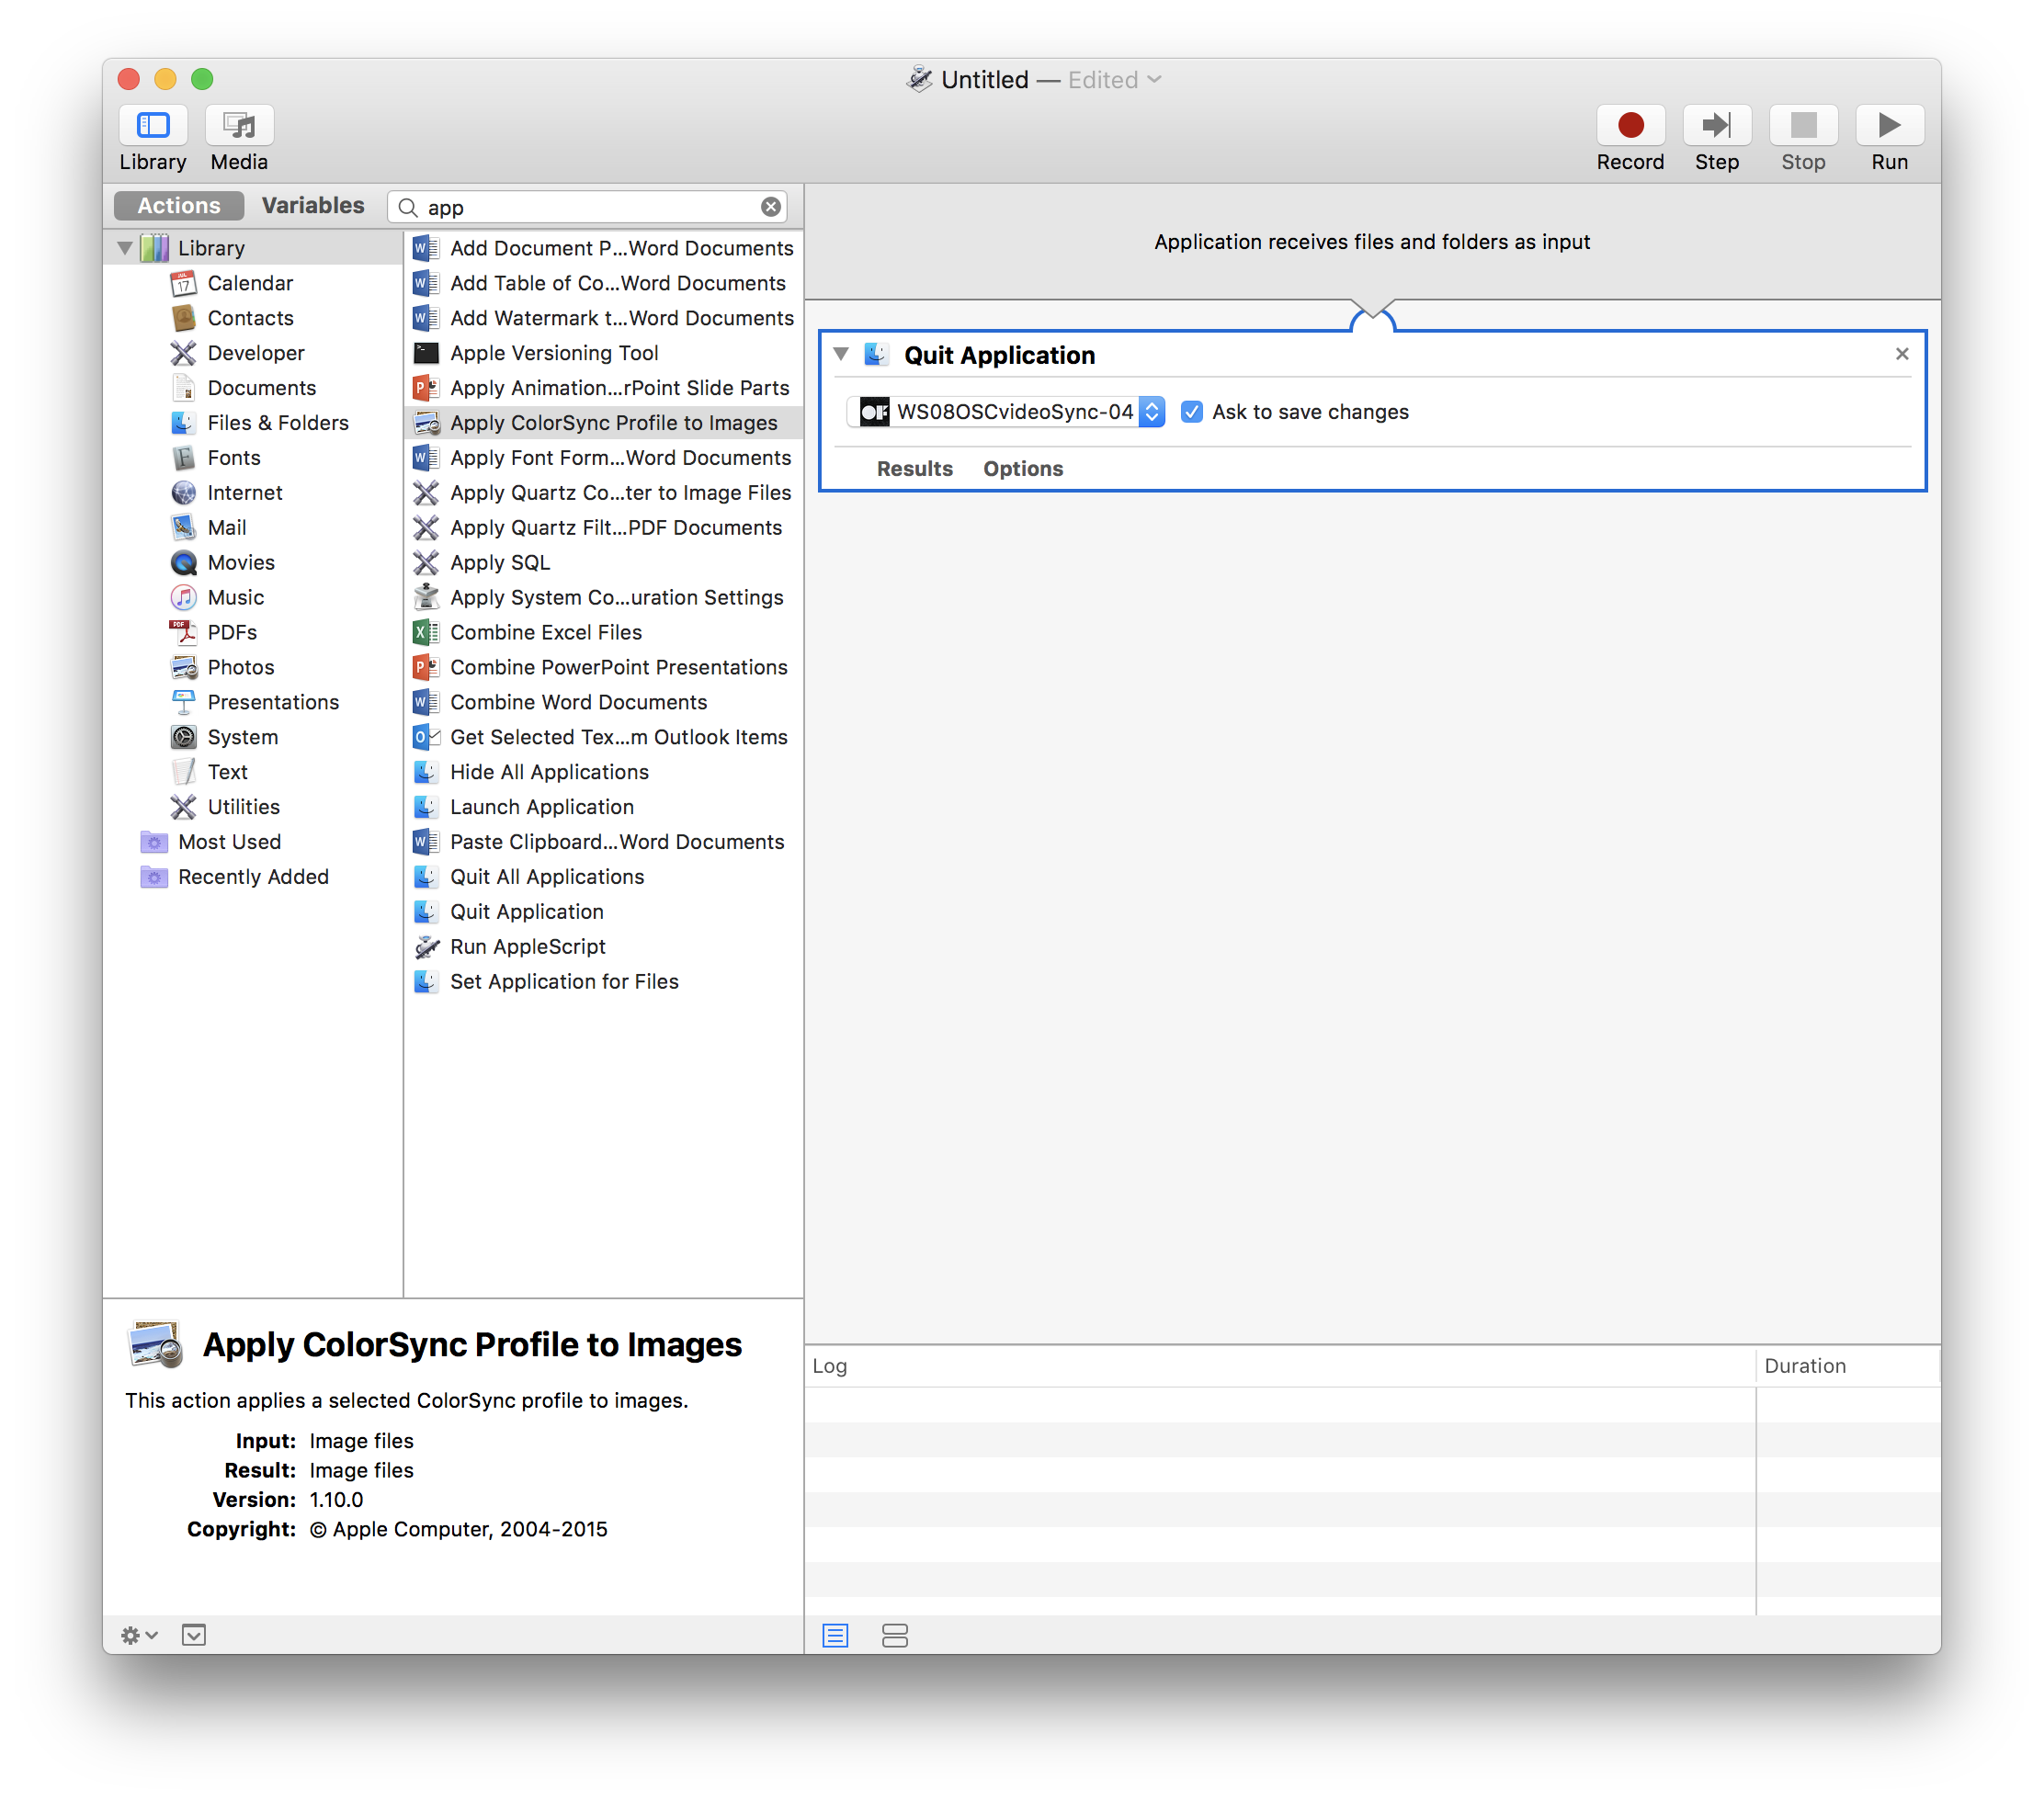
\includegraphics[width=70mm]{images/app-14.png}
                    \caption{結果}
                    \label{fig:21}
                \end{figure}
        \end{frame}

        \begin{frame}
            \frametitle{アプリの自動起動・終了}
                \begin{figure}[htb]
                    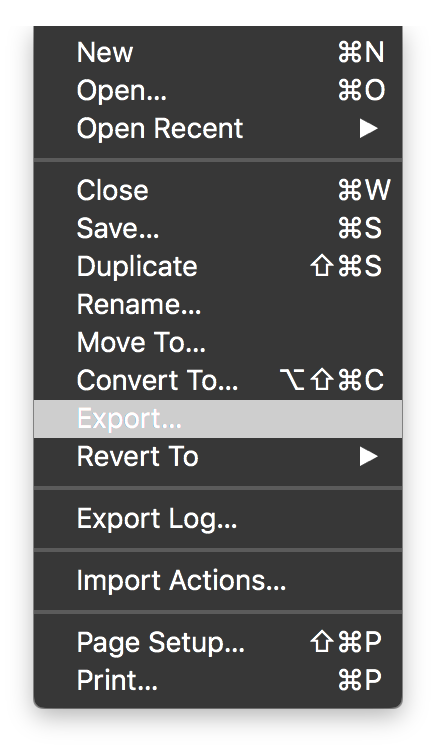
\includegraphics[width=20mm]{images/app-15.png}
                    \caption{ファイル>書き出し を選択}
                    \label{fig:22}
                \end{figure}
        \end{frame}

        \begin{frame}
            \frametitle{アプリの自動起動・終了}
                \begin{figure}[htb]
                    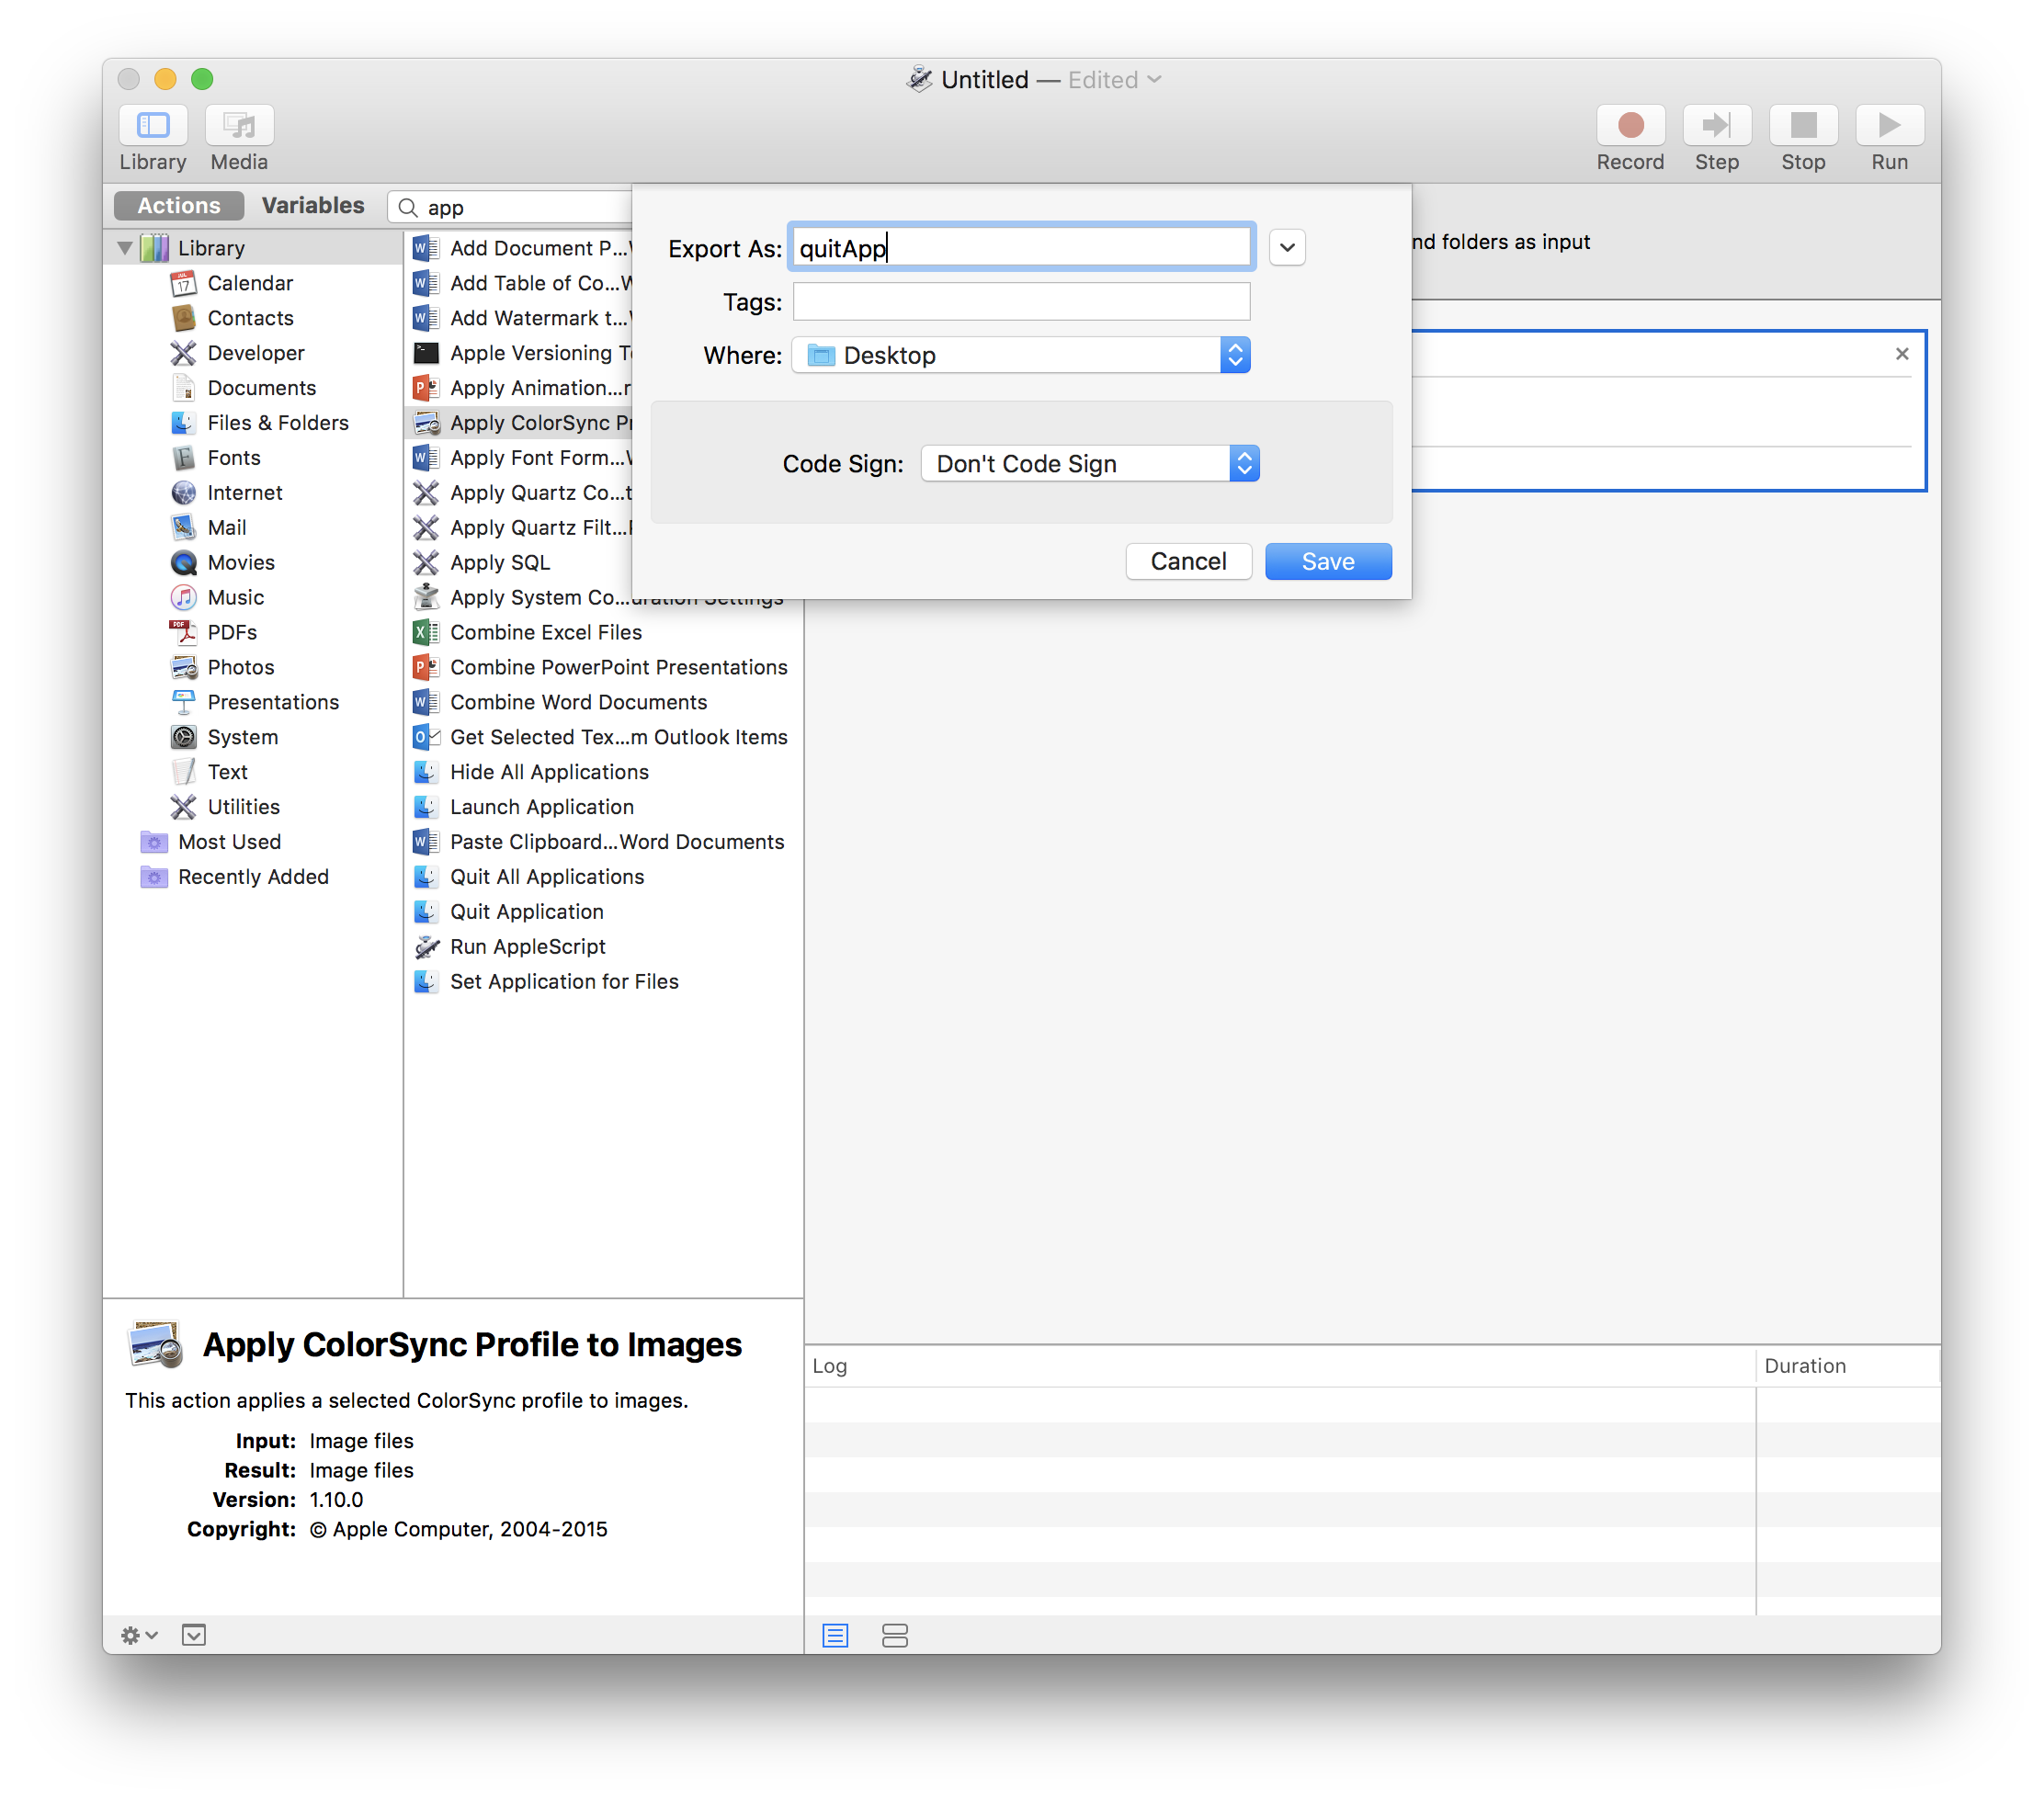
\includegraphics[width=70mm]{images/app-16.png}
                    \caption{書き出しアプリ名を決定}
                    \label{fig:23}
                \end{figure}
        \end{frame}

        \begin{frame}
            \frametitle{アプリの自動起動・終了}
                \begin{figure}[htb]
                    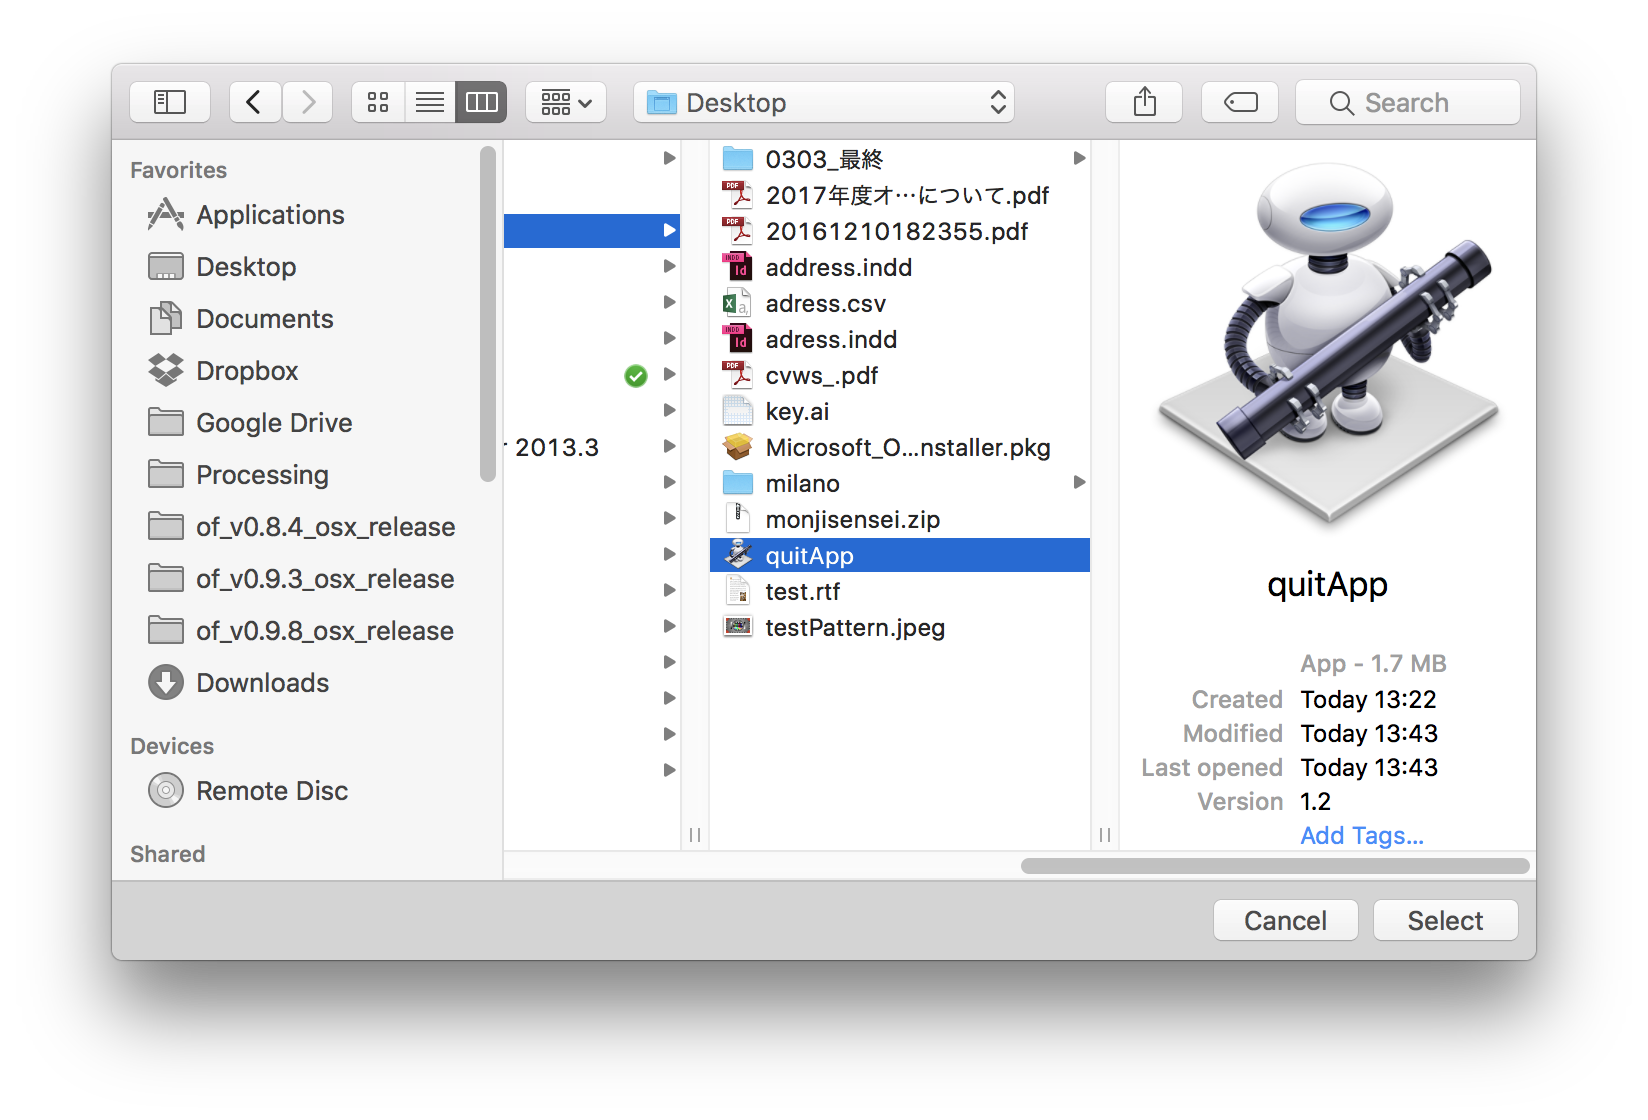
\includegraphics[width=70mm]{images/app-17.png}
                    \caption{カレンダーで開く制作したアプリを選択}
                    \label{fig:24}
                \end{figure}
        \end{frame}

        \begin{frame}
            \frametitle{アプリの自動起動・終了}
                \begin{figure}[htb]
                    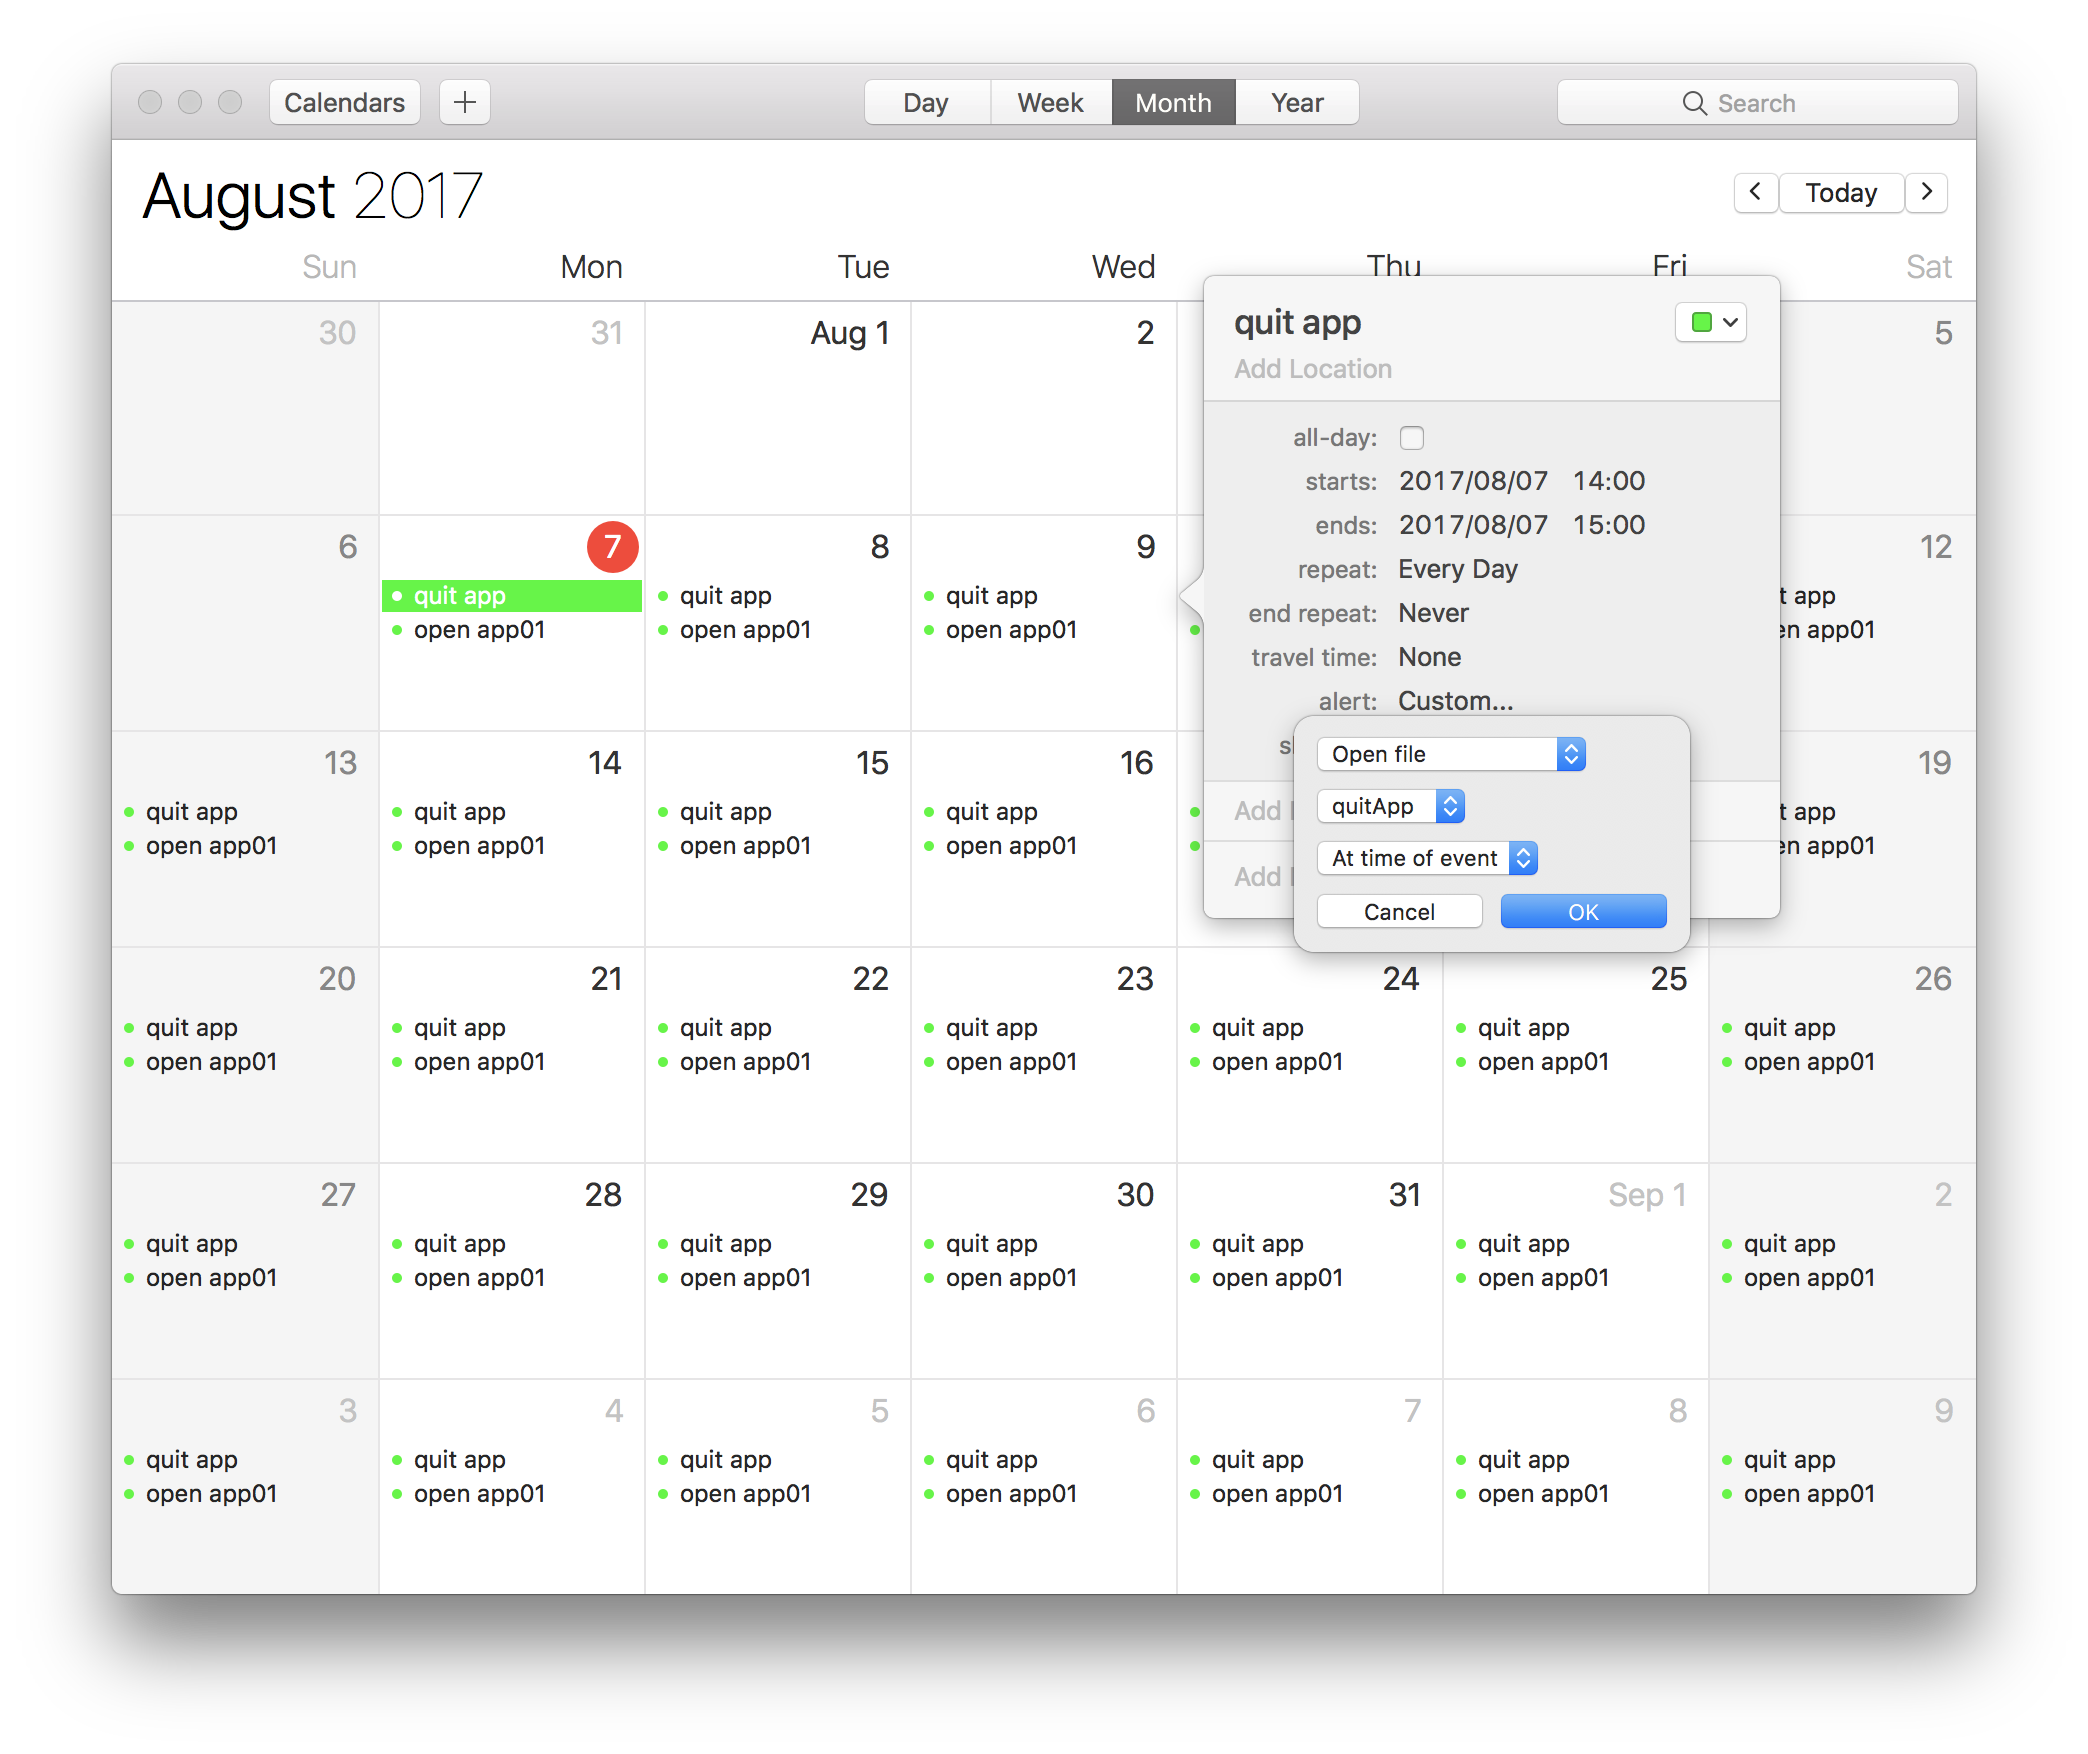
\includegraphics[width=70mm]{images/app-18.png}
                    \caption{結果}
                    \label{fig:25}
                \end{figure}
        \end{frame}

    \subsection{物理タイマーの利用}
        \begin{frame}
            \frametitle{物理タイマーの利用}
            \begin{block}{物理タイマーの意義}
                \begin{itemize}
                    \item 決まった時間に決まった装置を通電できる
                    \item 最もシンプル
                    \item 間接照明,Arduinoなど用途様々(ラズパイは不可)
                \end{itemize}
            \end{block}
        \end{frame}

        \begin{frame}
            \frametitle{物理タイマーの利用}
                \begin{figure}[htb]
                    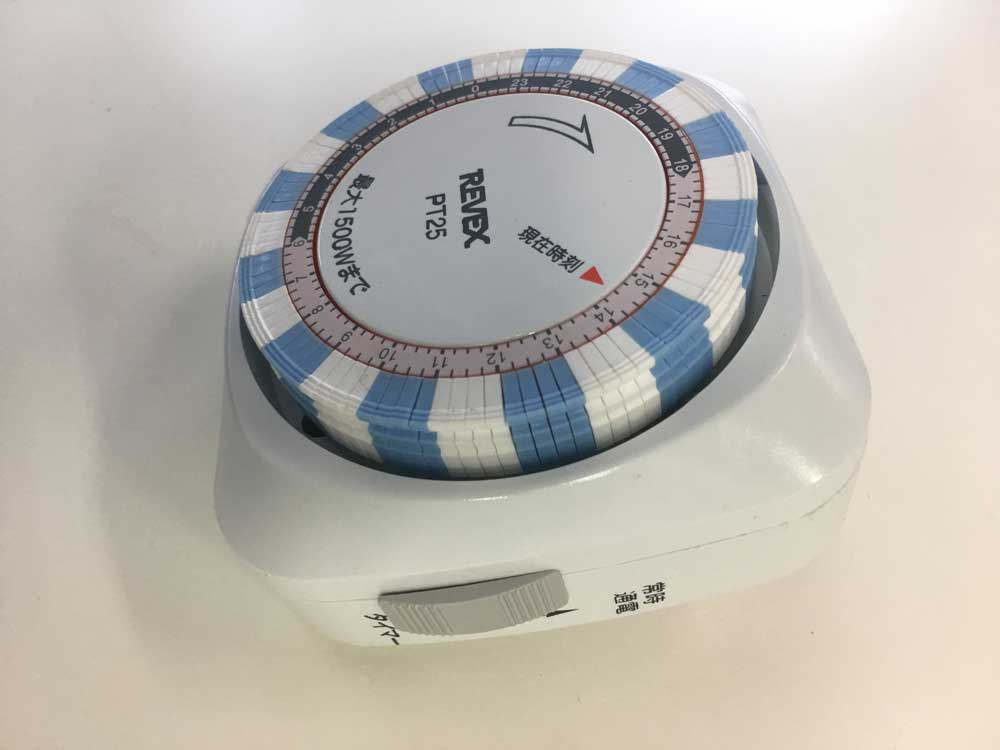
\includegraphics[width=70mm]{images/timer-1.jpg}
                    \caption{物理タイマー概観}
                    \label{fig:26}
                \end{figure}
        \end{frame}

        \begin{frame}
            \frametitle{物理タイマーの利用}
                \begin{figure}[htb]
                    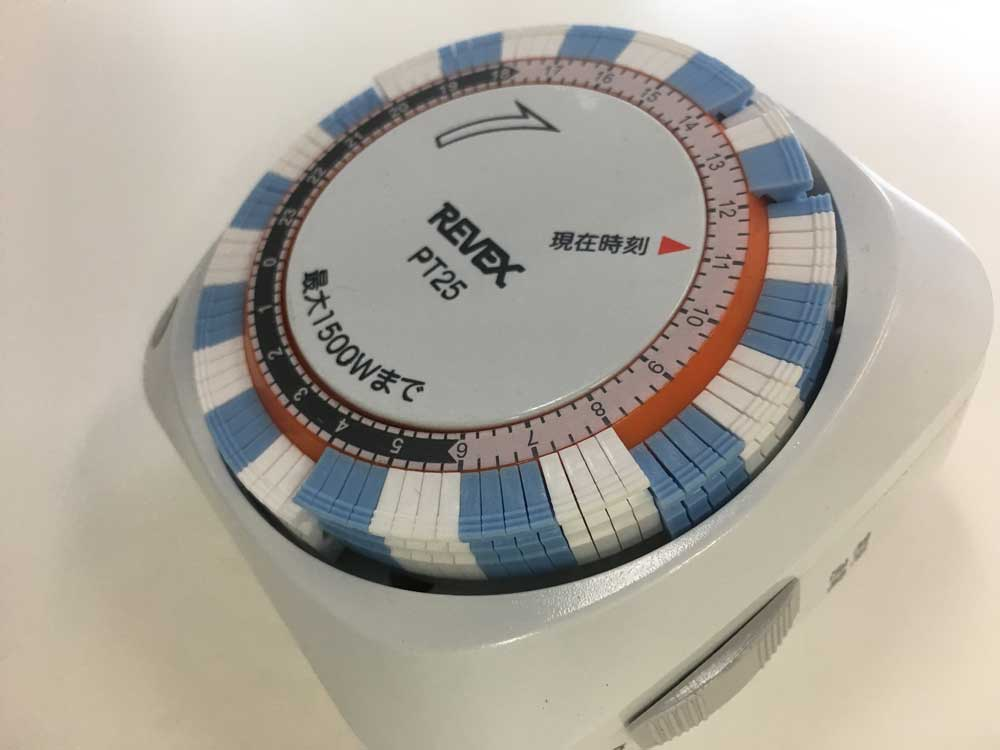
\includegraphics[width=70mm]{images/timer-2.jpg}
                    \caption{通電時間指定後}
                    \label{fig:27}
                \end{figure}
        \end{frame}
\end{document}

